\documentclass[a4paper]{book}
\usepackage{a4wide}
\usepackage{makeidx}
\usepackage{graphicx}
\usepackage{multicol}
\usepackage{float}
\usepackage{listings}
\usepackage{color}
\usepackage{textcomp}
\usepackage{alltt}
\usepackage{times}
\usepackage{ifpdf}
\ifpdf
\usepackage[pdftex,
            pagebackref=true,
            colorlinks=true,
            linkcolor=blue,
            unicode
           ]{hyperref}
\else
\usepackage[ps2pdf,
            pagebackref=true,
            colorlinks=true,
            linkcolor=blue,
            unicode
           ]{hyperref}
\usepackage{pspicture}
\fi
\usepackage[utf8]{inputenc}
\usepackage{doxygen}
\lstset{language=C++,inputencoding=utf8,basicstyle=\footnotesize,breaklines=true,breakatwhitespace=true,tabsize=8,numbers=left }
\makeindex
\setcounter{tocdepth}{3}
\renewcommand{\footrulewidth}{0.4pt}
\begin{document}
\hypersetup{pageanchor=false}
\begin{titlepage}
\vspace*{7cm}
\begin{center}
{\Large Simple3D }\\
\vspace*{1cm}
{\large Generated by Doxygen 1.6.3}\\
\vspace*{0.5cm}
{\small Sat Sep 18 06:56:04 2010}\\
\end{center}
\end{titlepage}
\clearemptydoublepage
\pagenumbering{roman}
\tableofcontents
\clearemptydoublepage
\pagenumbering{arabic}
\hypersetup{pageanchor=true}
\chapter{Todo List}
\label{todo}
\hypertarget{todo}{}
\label{todo__todo000001}
\hypertarget{todo__todo000001}{}
 
\begin{DoxyDescription}
\item[Member \hyperlink{class_s3_d_mesh_ad1de35530a123dbb515e37afc8ecc0e3}{S3DMesh::scale}(double fx, double fy, double fz) ]Fix this thing. Its fucked up yet. 
\end{DoxyDescription}

\label{todo__todo000002}
\hypertarget{todo__todo000002}{}
 
\begin{DoxyDescription}
\item[Member \hyperlink{class_s3_d_triangle_a0808a047e513fb2322e3fc6465c7c011}{S3DTriangle::scale}(double fx, double fy, double fz) ]Currently this works for stand-\/alone triangles, but not for triangles belonging to \hyperlink{class_s3_d_mesh}{S3DMesh}. 
\end{DoxyDescription}
\chapter{Class Index}
\section{Class Hierarchy}
This inheritance list is sorted roughly, but not completely, alphabetically:\begin{DoxyCompactList}
\item \contentsline{section}{Point}{\pageref{struct_point}}{}
\item \contentsline{section}{S3DColor}{\pageref{struct_s3_d_color}}{}
\item \contentsline{section}{S3DPoint}{\pageref{class_s3_d_point}}{}
\item \contentsline{section}{S3DPrimitive}{\pageref{class_s3_d_primitive}}{}
\begin{DoxyCompactList}
\item \contentsline{section}{S3DCube}{\pageref{class_s3_d_cube}}{}
\item \contentsline{section}{S3DLine}{\pageref{class_s3_d_line}}{}
\item \contentsline{section}{S3DMesh}{\pageref{class_s3_d_mesh}}{}
\item \contentsline{section}{S3DRect}{\pageref{class_s3_d_rect}}{}
\item \contentsline{section}{S3DTetraeder}{\pageref{class_s3_d_tetraeder}}{}
\item \contentsline{section}{S3DTriangle}{\pageref{class_s3_d_triangle}}{}
\end{DoxyCompactList}
\item \contentsline{section}{S3DZBuffer}{\pageref{class_s3_d_z_buffer}}{}
\item \contentsline{section}{Simple3D}{\pageref{class_simple3_d}}{}
\end{DoxyCompactList}

\chapter{Class Index}
\section{Class List}
Here are the classes, structs, unions and interfaces with brief descriptions:\begin{DoxyCompactList}
\item\contentsline{section}{\hyperlink{struct_point}{Point} }{\pageref{struct_point}}{}
\item\contentsline{section}{\hyperlink{struct_s3_d_color}{S3DColor} }{\pageref{struct_s3_d_color}}{}
\item\contentsline{section}{\hyperlink{class_s3_d_cube}{S3DCube} }{\pageref{class_s3_d_cube}}{}
\item\contentsline{section}{\hyperlink{class_s3_d_line}{S3DLine} (Class for the line-\/primitive in S3D )}{\pageref{class_s3_d_line}}{}
\item\contentsline{section}{\hyperlink{class_s3_d_mesh}{S3DMesh} (This class is used to load a collection of triangles to use it as an entity )}{\pageref{class_s3_d_mesh}}{}
\item\contentsline{section}{\hyperlink{class_s3_d_point}{S3DPoint} (This class is used for representing 3d-\/coordinates )}{\pageref{class_s3_d_point}}{}
\item\contentsline{section}{\hyperlink{class_s3_d_primitive}{S3DPrimitive} (This class is the base of all primitives in S3D )}{\pageref{class_s3_d_primitive}}{}
\item\contentsline{section}{\hyperlink{class_s3_d_rect}{S3DRect} }{\pageref{class_s3_d_rect}}{}
\item\contentsline{section}{\hyperlink{class_s3_d_tetraeder}{S3DTetraeder} }{\pageref{class_s3_d_tetraeder}}{}
\item\contentsline{section}{\hyperlink{class_s3_d_triangle}{S3DTriangle} (This is the main primitive actually used )}{\pageref{class_s3_d_triangle}}{}
\item\contentsline{section}{\hyperlink{class_s3_d_z_buffer}{S3DZBuffer} (This class is responsible for z-\/buffering )}{\pageref{class_s3_d_z_buffer}}{}
\item\contentsline{section}{\hyperlink{class_simple3_d}{Simple3D} (This class is the main class of the engine )}{\pageref{class_simple3_d}}{}
\end{DoxyCompactList}

\chapter{File Index}
\section{File List}
Here is a list of all files with brief descriptions:\begin{DoxyCompactList}
\item\contentsline{section}{\hyperlink{global_8h}{global.h} (Contains basic includes (including platform-\/dependent) and definitions for the whole library )}{\pageref{global_8h}}{}
\item\contentsline{section}{\hyperlink{main_8cpp}{main.cpp} }{\pageref{main_8cpp}}{}
\item\contentsline{section}{\hyperlink{_s3_d_cube_8cpp}{S3DCube.cpp} }{\pageref{_s3_d_cube_8cpp}}{}
\item\contentsline{section}{\hyperlink{_s3_d_cube_8h}{S3DCube.h} }{\pageref{_s3_d_cube_8h}}{}
\item\contentsline{section}{\hyperlink{_s3_d_line_8cpp}{S3DLine.cpp} (Contains the implementation of the S3DLine-\/Primitive )}{\pageref{_s3_d_line_8cpp}}{}
\item\contentsline{section}{\hyperlink{_s3_d_line_8h}{S3DLine.h} (Contains the class-\/definition (and getter and setter) for \hyperlink{class_s3_d_line}{S3DLine} )}{\pageref{_s3_d_line_8h}}{}
\item\contentsline{section}{\hyperlink{_s3_d_mesh_8cpp}{S3DMesh.cpp} }{\pageref{_s3_d_mesh_8cpp}}{}
\item\contentsline{section}{\hyperlink{_s3_d_mesh_8h}{S3DMesh.h} }{\pageref{_s3_d_mesh_8h}}{}
\item\contentsline{section}{\hyperlink{_s3_d_point_8cpp}{S3DPoint.cpp} }{\pageref{_s3_d_point_8cpp}}{}
\item\contentsline{section}{\hyperlink{_s3_d_point_8h}{S3DPoint.h} }{\pageref{_s3_d_point_8h}}{}
\item\contentsline{section}{\hyperlink{_s3_d_primitive_8cpp}{S3DPrimitive.cpp} }{\pageref{_s3_d_primitive_8cpp}}{}
\item\contentsline{section}{\hyperlink{_s3_d_primitive_8h}{S3DPrimitive.h} }{\pageref{_s3_d_primitive_8h}}{}
\item\contentsline{section}{\hyperlink{_s3_d_rect_8cpp}{S3DRect.cpp} }{\pageref{_s3_d_rect_8cpp}}{}
\item\contentsline{section}{\hyperlink{_s3_d_rect_8h}{S3DRect.h} }{\pageref{_s3_d_rect_8h}}{}
\item\contentsline{section}{\hyperlink{_s3_d_tetraeder_8cpp}{S3DTetraeder.cpp} }{\pageref{_s3_d_tetraeder_8cpp}}{}
\item\contentsline{section}{\hyperlink{_s3_d_tetraeder_8h}{S3DTetraeder.h} }{\pageref{_s3_d_tetraeder_8h}}{}
\item\contentsline{section}{\hyperlink{_s3_d_triangle_8cpp}{S3DTriangle.cpp} }{\pageref{_s3_d_triangle_8cpp}}{}
\item\contentsline{section}{\hyperlink{_s3_d_triangle_8h}{S3DTriangle.h} }{\pageref{_s3_d_triangle_8h}}{}
\item\contentsline{section}{\hyperlink{_s3_d_z_buffer_8cpp}{S3DZBuffer.cpp} }{\pageref{_s3_d_z_buffer_8cpp}}{}
\item\contentsline{section}{\hyperlink{_s3_d_z_buffer_8h}{S3DZBuffer.h} }{\pageref{_s3_d_z_buffer_8h}}{}
\item\contentsline{section}{\hyperlink{_simple3_d_8cpp}{Simple3D.cpp} }{\pageref{_simple3_d_8cpp}}{}
\item\contentsline{section}{\hyperlink{_simple3_d_8h}{Simple3D.h} }{\pageref{_simple3_d_8h}}{}
\item\contentsline{section}{\hyperlink{types_8h}{types.h} }{\pageref{types_8h}}{}
\item\contentsline{section}{\hyperlink{_write_demo_mesh_8c}{WriteDemoMesh.c} }{\pageref{_write_demo_mesh_8c}}{}
\end{DoxyCompactList}

\chapter{Class Documentation}
\hypertarget{struct_point}{
\section{Point Struct Reference}
\label{struct_point}\index{Point@{Point}}
}
\subsection*{Public Attributes}
\begin{DoxyCompactItemize}
\item 
double \hyperlink{struct_point_ab99c56589bc8ad5fa5071387110a5bc7}{x}
\item 
double \hyperlink{struct_point_afa38be143ae800e6ad69ce8ed4df62d8}{y}
\item 
double \hyperlink{struct_point_a05ba3b1dfcb19430582ae953cbbfbded}{z}
\end{DoxyCompactItemize}


\subsection{Member Data Documentation}
\hypertarget{struct_point_ab99c56589bc8ad5fa5071387110a5bc7}{
\index{Point@{Point}!x@{x}}
\index{x@{x}!Point@{Point}}
\subsubsection[{x}]{\setlength{\rightskip}{0pt plus 5cm}double {\bf Point::x}}}
\label{struct_point_ab99c56589bc8ad5fa5071387110a5bc7}
\hypertarget{struct_point_afa38be143ae800e6ad69ce8ed4df62d8}{
\index{Point@{Point}!y@{y}}
\index{y@{y}!Point@{Point}}
\subsubsection[{y}]{\setlength{\rightskip}{0pt plus 5cm}double {\bf Point::y}}}
\label{struct_point_afa38be143ae800e6ad69ce8ed4df62d8}
\hypertarget{struct_point_a05ba3b1dfcb19430582ae953cbbfbded}{
\index{Point@{Point}!z@{z}}
\index{z@{z}!Point@{Point}}
\subsubsection[{z}]{\setlength{\rightskip}{0pt plus 5cm}double {\bf Point::z}}}
\label{struct_point_a05ba3b1dfcb19430582ae953cbbfbded}


The documentation for this struct was generated from the following file:\begin{DoxyCompactItemize}
\item 
\hyperlink{_write_demo_mesh_8c}{WriteDemoMesh.c}\end{DoxyCompactItemize}

\hypertarget{struct_s3_d_color}{
\section{S3DColor Struct Reference}
\label{struct_s3_d_color}\index{S3DColor@{S3DColor}}
}


{\ttfamily \#include $<$types.h$>$}

\subsection*{Public Attributes}
\begin{DoxyCompactItemize}
\item 
\hypertarget{struct_s3_d_color_a4a7329c346d7745fd46b81a5d1cac393}{
unsigned char {\bfseries r}}
\label{struct_s3_d_color_a4a7329c346d7745fd46b81a5d1cac393}

\item 
\hypertarget{struct_s3_d_color_a6f926b101765a5b848dfb5acdce1f1a4}{
unsigned char {\bfseries g}}
\label{struct_s3_d_color_a6f926b101765a5b848dfb5acdce1f1a4}

\item 
\hypertarget{struct_s3_d_color_af03f6858e55796ca988a17b15c2284b3}{
unsigned char {\bfseries b}}
\label{struct_s3_d_color_af03f6858e55796ca988a17b15c2284b3}

\end{DoxyCompactItemize}


\subsection{Detailed Description}
\hyperlink{types_8h_source}{types.h} -\/ defines basic types and structures of \hyperlink{class_simple3_d}{Simple3D} 

The documentation for this struct was generated from the following file:\begin{DoxyCompactItemize}
\item 
Simple3D/types.h\end{DoxyCompactItemize}

\hypertarget{class_s3_d_cube}{
\section{S3DCube Class Reference}
\label{class_s3_d_cube}\index{S3DCube@{S3DCube}}
}


{\ttfamily \#include $<$S3DCube.h$>$}

Inheritance diagram for S3DCube:\begin{figure}[H]
\begin{center}
\leavevmode
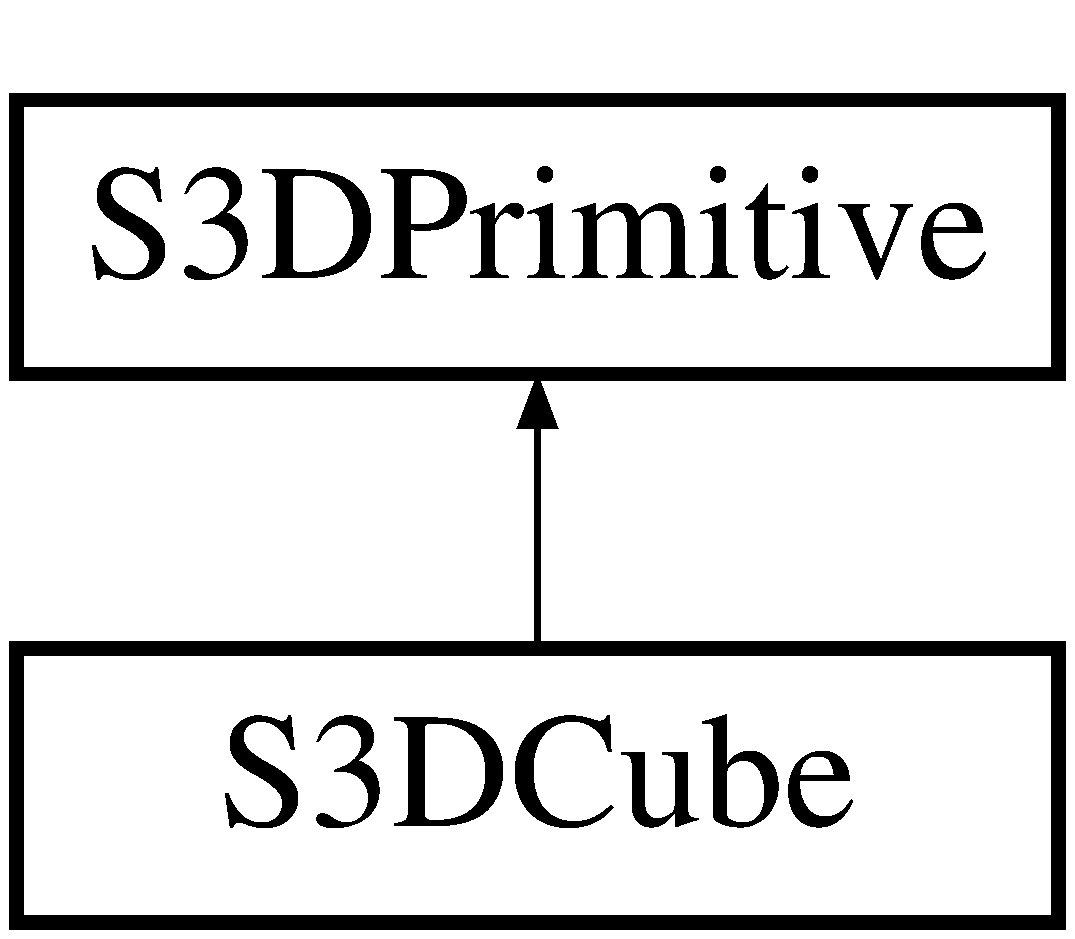
\includegraphics[height=2cm]{class_s3_d_cube}
\end{center}
\end{figure}
\subsection*{Public Member Functions}
\begin{DoxyCompactItemize}
\item 
\hyperlink{class_s3_d_cube_a071b56f85b667b74d0056d0d554d3647}{S3DCube} (\hyperlink{class_s3_d_rect}{S3DRect} $\ast$s\mbox{[}6\mbox{]})
\item 
\hyperlink{class_s3_d_cube_a6bda81748dd5c23028611bf2863bcd69}{S3DCube} (\hyperlink{class_s3_d_point}{S3DPoint} edges\mbox{[}8\mbox{]})
\item 
\hyperlink{class_s3_d_cube_a96e5dcdd93eb3fcdcbadbce2f52e1890}{S3DCube} (\hyperlink{class_s3_d_point}{S3DPoint} a, \hyperlink{class_s3_d_point}{S3DPoint} b, \hyperlink{class_s3_d_point}{S3DPoint} c, \hyperlink{class_s3_d_point}{S3DPoint} d, \hyperlink{class_s3_d_point}{S3DPoint} e, \hyperlink{class_s3_d_point}{S3DPoint} f, \hyperlink{class_s3_d_point}{S3DPoint} g, \hyperlink{class_s3_d_point}{S3DPoint} h)
\item 
void \hyperlink{class_s3_d_cube_ab21a1988528297602452984f8a3c093e}{move} (double dx, double dy, double dz)
\begin{DoxyCompactList}\small\item\em Virtual method. Implementations are responsible for moving the primitive. \item\end{DoxyCompactList}\item 
void \hyperlink{class_s3_d_cube_a2e574649ca6ddd805c5ecdb7932f3ac1}{rotate} (double rx, double ry, double rz, \hyperlink{class_s3_d_point}{S3DPoint} $\ast$anchor=NULL)
\begin{DoxyCompactList}\small\item\em Virtual method. Implementations are responsible for rotating the primitive. \item\end{DoxyCompactList}\item 
void \hyperlink{class_s3_d_cube_a1e66a1dab7e99328fab61c2c86da7ba5}{draw} (\hyperlink{types_8h_a25c0773a29204332721bde1b164d0b84}{S3DDevice} $\ast$d, \hyperlink{types_8h_a4afc89c514af26434688c7e8b382ba5e}{S3DSurface} w, \hyperlink{types_8h_a46f30693e0040340e595d8228cc31779}{S3DContext} g)
\item 
void \hyperlink{class_s3_d_cube_a9c48875a16cc0ace3a3092e98663b785}{setColor} (unsigned long c)
\begin{DoxyCompactList}\small\item\em Sets the color of the primitive. \item\end{DoxyCompactList}\item 
unsigned long \hyperlink{class_s3_d_cube_ab856b6fa4c1b72be7d2d7b79e26f3c38}{getColor} ()
\begin{DoxyCompactList}\small\item\em Returns the color of the primitive. \item\end{DoxyCompactList}\item 
double \hyperlink{class_s3_d_cube_a4ac1d080b330d6b69d24097f746ddd4c}{getZ} ()
\begin{DoxyCompactList}\small\item\em Virtual method. Implementations are responsible for return some z-\/Value the primitive. \item\end{DoxyCompactList}\end{DoxyCompactItemize}


\subsection{Constructor \& Destructor Documentation}
\hypertarget{class_s3_d_cube_a071b56f85b667b74d0056d0d554d3647}{
\index{S3DCube@{S3DCube}!S3DCube@{S3DCube}}
\index{S3DCube@{S3DCube}!S3DCube@{S3DCube}}
\subsubsection[{S3DCube}]{\setlength{\rightskip}{0pt plus 5cm}S3DCube::S3DCube ({\bf S3DRect} $\ast$ {\em s}\mbox{[}6\mbox{]})}}
\label{class_s3_d_cube_a071b56f85b667b74d0056d0d554d3647}
\hypertarget{class_s3_d_cube_a6bda81748dd5c23028611bf2863bcd69}{
\index{S3DCube@{S3DCube}!S3DCube@{S3DCube}}
\index{S3DCube@{S3DCube}!S3DCube@{S3DCube}}
\subsubsection[{S3DCube}]{\setlength{\rightskip}{0pt plus 5cm}S3DCube::S3DCube ({\bf S3DPoint} {\em edges}\mbox{[}8\mbox{]})}}
\label{class_s3_d_cube_a6bda81748dd5c23028611bf2863bcd69}
\hypertarget{class_s3_d_cube_a96e5dcdd93eb3fcdcbadbce2f52e1890}{
\index{S3DCube@{S3DCube}!S3DCube@{S3DCube}}
\index{S3DCube@{S3DCube}!S3DCube@{S3DCube}}
\subsubsection[{S3DCube}]{\setlength{\rightskip}{0pt plus 5cm}S3DCube::S3DCube ({\bf S3DPoint} {\em a}, \/  {\bf S3DPoint} {\em b}, \/  {\bf S3DPoint} {\em c}, \/  {\bf S3DPoint} {\em d}, \/  {\bf S3DPoint} {\em e}, \/  {\bf S3DPoint} {\em f}, \/  {\bf S3DPoint} {\em g}, \/  {\bf S3DPoint} {\em h})}}
\label{class_s3_d_cube_a96e5dcdd93eb3fcdcbadbce2f52e1890}


\subsection{Member Function Documentation}
\hypertarget{class_s3_d_cube_a1e66a1dab7e99328fab61c2c86da7ba5}{
\index{S3DCube@{S3DCube}!draw@{draw}}
\index{draw@{draw}!S3DCube@{S3DCube}}
\subsubsection[{draw}]{\setlength{\rightskip}{0pt plus 5cm}void S3DCube::draw ({\bf S3DDevice} $\ast$ {\em d}, \/  {\bf S3DSurface} {\em w}, \/  {\bf S3DContext} {\em g})}}
\label{class_s3_d_cube_a1e66a1dab7e99328fab61c2c86da7ba5}
\hypertarget{class_s3_d_cube_ab856b6fa4c1b72be7d2d7b79e26f3c38}{
\index{S3DCube@{S3DCube}!getColor@{getColor}}
\index{getColor@{getColor}!S3DCube@{S3DCube}}
\subsubsection[{getColor}]{\setlength{\rightskip}{0pt plus 5cm}unsigned long S3DCube::getColor ()}}
\label{class_s3_d_cube_ab856b6fa4c1b72be7d2d7b79e26f3c38}


Returns the color of the primitive. 



Reimplemented from \hyperlink{class_s3_d_primitive_a4102845e7754e44c51a87c0fcb391c73}{S3DPrimitive}.

\hypertarget{class_s3_d_cube_a4ac1d080b330d6b69d24097f746ddd4c}{
\index{S3DCube@{S3DCube}!getZ@{getZ}}
\index{getZ@{getZ}!S3DCube@{S3DCube}}
\subsubsection[{getZ}]{\setlength{\rightskip}{0pt plus 5cm}double S3DCube::getZ ()\hspace{0.3cm}{\ttfamily  \mbox{[}virtual\mbox{]}}}}
\label{class_s3_d_cube_a4ac1d080b330d6b69d24097f746ddd4c}


Virtual method. Implementations are responsible for return some z-\/Value the primitive. 



Implements \hyperlink{class_s3_d_primitive_ab5b06d3a8e83216cc42554bb78afd2d9}{S3DPrimitive}.

\hypertarget{class_s3_d_cube_ab21a1988528297602452984f8a3c093e}{
\index{S3DCube@{S3DCube}!move@{move}}
\index{move@{move}!S3DCube@{S3DCube}}
\subsubsection[{move}]{\setlength{\rightskip}{0pt plus 5cm}void S3DCube::move (double {\em dx}, \/  double {\em dy}, \/  double {\em dz})\hspace{0.3cm}{\ttfamily  \mbox{[}virtual\mbox{]}}}}
\label{class_s3_d_cube_ab21a1988528297602452984f8a3c093e}


Virtual method. Implementations are responsible for moving the primitive. 



Implements \hyperlink{class_s3_d_primitive_a73a178ec2e1aa8e95f01baf0552724a9}{S3DPrimitive}.

\hypertarget{class_s3_d_cube_a2e574649ca6ddd805c5ecdb7932f3ac1}{
\index{S3DCube@{S3DCube}!rotate@{rotate}}
\index{rotate@{rotate}!S3DCube@{S3DCube}}
\subsubsection[{rotate}]{\setlength{\rightskip}{0pt plus 5cm}void S3DCube::rotate (double {\em rx}, \/  double {\em ry}, \/  double {\em rz}, \/  {\bf S3DPoint} $\ast$ {\em anchor} = {\ttfamily NULL})\hspace{0.3cm}{\ttfamily  \mbox{[}virtual\mbox{]}}}}
\label{class_s3_d_cube_a2e574649ca6ddd805c5ecdb7932f3ac1}


Virtual method. Implementations are responsible for rotating the primitive. 



Implements \hyperlink{class_s3_d_primitive_a23eb36b6bd48643e8f7be4b950592d9e}{S3DPrimitive}.

\hypertarget{class_s3_d_cube_a9c48875a16cc0ace3a3092e98663b785}{
\index{S3DCube@{S3DCube}!setColor@{setColor}}
\index{setColor@{setColor}!S3DCube@{S3DCube}}
\subsubsection[{setColor}]{\setlength{\rightskip}{0pt plus 5cm}void S3DCube::setColor (unsigned long {\em c})}}
\label{class_s3_d_cube_a9c48875a16cc0ace3a3092e98663b785}


Sets the color of the primitive. 


\begin{DoxyParams}{Parameters}
\item[\mbox{$\leftarrow$} {\em c}]The color as unsigned long (as produced by RGB-\/macro), the primitive will get. \end{DoxyParams}


Reimplemented from \hyperlink{class_s3_d_primitive_a1c8f036193987522bdfb6a49b9b74000}{S3DPrimitive}.



The documentation for this class was generated from the following files:\begin{DoxyCompactItemize}
\item 
\hyperlink{_s3_d_cube_8h}{S3DCube.h}\item 
\hyperlink{_s3_d_cube_8cpp}{S3DCube.cpp}\end{DoxyCompactItemize}

\hypertarget{class_s3_d_line}{
\section{S3DLine Class Reference}
\label{class_s3_d_line}\index{S3DLine@{S3DLine}}
}


Class for the line-\/primitive in S3D.  




{\ttfamily \#include $<$S3DLine.h$>$}

Inheritance diagram for S3DLine:\begin{figure}[H]
\begin{center}
\leavevmode
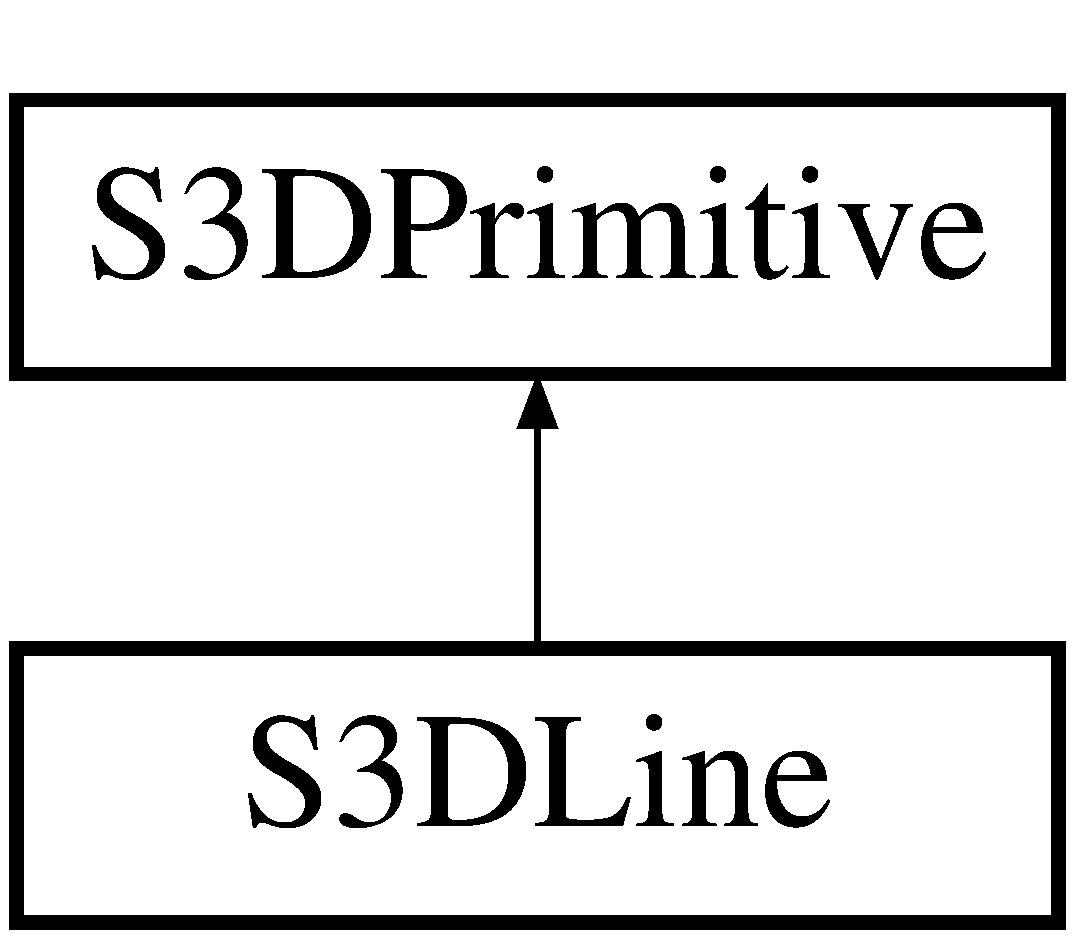
\includegraphics[height=2cm]{class_s3_d_line}
\end{center}
\end{figure}
\subsection*{Public Member Functions}
\begin{DoxyCompactItemize}
\item 
\hyperlink{class_s3_d_line_ae6eeda40b82f27193b1d1165a8fb3e63}{S3DLine} (\hyperlink{class_s3_d_point}{S3DPoint} a, \hyperlink{class_s3_d_point}{S3DPoint} b)
\begin{DoxyCompactList}\small\item\em Creates a line between two (3D-\/)Points. \item\end{DoxyCompactList}\item 
void \hyperlink{class_s3_d_line_aa7732c2d83fecb5d9934863d0e7875c1}{draw} (S3DDevice $\ast$disp, S3DSurface window, S3DContext gc, \hyperlink{class_s3_d_z_buffer}{S3DZBuffer} $\ast$zbuffer)
\begin{DoxyCompactList}\small\item\em Draws the line. \item\end{DoxyCompactList}\item 
void \hyperlink{class_s3_d_line_a38203e499c32f14ff5da3b7c17861881}{move} (double dx, double dy, double dz)
\begin{DoxyCompactList}\small\item\em Moves the line (translates it) relative to its coordinates. \item\end{DoxyCompactList}\item 
void \hyperlink{class_s3_d_line_a49a646c9b24de7847eb45cac31dd3a27}{scale} (double fx, double fy, double fz)
\begin{DoxyCompactList}\small\item\em Scales the line. \item\end{DoxyCompactList}\item 
void \hyperlink{class_s3_d_line_a4d23495df2c8f45855d8b80d30b01d30}{rotate} (double rx, double ry, double rz, \hyperlink{class_s3_d_point}{S3DPoint} $\ast$anchor=NULL)
\begin{DoxyCompactList}\small\item\em Rotates the line around its center or another anchor point. \item\end{DoxyCompactList}\item 
double \hyperlink{class_s3_d_line_a72aabdbb4d3d0c3ea36f5fda7b059f6a}{getZ} ()
\begin{DoxyCompactList}\small\item\em Returns the z-\/coordinate for the center of the line. \item\end{DoxyCompactList}\item 
void \hyperlink{class_s3_d_line_a9feaf056477e858a7b0248a7b5cdd222}{setColor} (unsigned long c)
\begin{DoxyCompactList}\small\item\em Sets the color of the line. \item\end{DoxyCompactList}\item 
unsigned long \hyperlink{class_s3_d_line_a62b49873ae3356cf997ca1fd87a1b7de}{getColor} ()
\begin{DoxyCompactList}\small\item\em Returns the color of the line. \item\end{DoxyCompactList}\item 
void \hyperlink{class_s3_d_line_a3b973e5206d4bed73b797b4c5afe8dec}{setProjected} (bool p)
\begin{DoxyCompactList}\small\item\em Setting the coordinate mode to projected coordinates. \item\end{DoxyCompactList}\end{DoxyCompactItemize}


\subsection{Detailed Description}
Class for the line-\/primitive in S3D. This class implements three-\/dimensional lines as the basis of all other primitives in S3D The line is the only primitive that is drawn using platform-\/dependent functions, all superior primitives will use this class to draw themselves. 

\subsection{Constructor \& Destructor Documentation}
\hypertarget{class_s3_d_line_ae6eeda40b82f27193b1d1165a8fb3e63}{
\index{S3DLine@{S3DLine}!S3DLine@{S3DLine}}
\index{S3DLine@{S3DLine}!S3DLine@{S3DLine}}
\subsubsection[{S3DLine}]{\setlength{\rightskip}{0pt plus 5cm}S3DLine::S3DLine ({\bf S3DPoint} {\em a}, \/  {\bf S3DPoint} {\em b})}}
\label{class_s3_d_line_ae6eeda40b82f27193b1d1165a8fb3e63}


Creates a line between two (3D-\/)Points. 


\begin{DoxyParams}{Parameters}
\item[\mbox{$\leftarrow$} {\em a}]First endpoint of the line \item[\mbox{$\leftarrow$} {\em b}]Second endpoint of the line \end{DoxyParams}


\subsection{Member Function Documentation}
\hypertarget{class_s3_d_line_aa7732c2d83fecb5d9934863d0e7875c1}{
\index{S3DLine@{S3DLine}!draw@{draw}}
\index{draw@{draw}!S3DLine@{S3DLine}}
\subsubsection[{draw}]{\setlength{\rightskip}{0pt plus 5cm}void S3DLine::draw (S3DDevice $\ast$ {\em disp}, \/  S3DSurface {\em window}, \/  S3DContext {\em gc}, \/  {\bf S3DZBuffer} $\ast$ {\em zbuffer})\hspace{0.3cm}{\ttfamily  \mbox{[}virtual\mbox{]}}}}
\label{class_s3_d_line_aa7732c2d83fecb5d9934863d0e7875c1}


Draws the line. 


\begin{DoxyParams}{Parameters}
\item[\mbox{$\leftarrow$} {\em disp}]The display device, the line will be drawn to \item[\mbox{$\leftarrow$} {\em window}]The surface, the line will be drawn to \item[\mbox{$\leftarrow$} {\em gc}]The context, the line will be drawn to \item[{\em zbuffer}]Pointer to the S3DZBuffer-\/Instance of the Simple3D-\/Instance.\end{DoxyParams}
This method is used to draw the line on screen, by using the platform-\/specific way of drawing points on some sort of screen. The meaning and neccessity of disp, window and gc may vary between different platforms 

Implements \hyperlink{class_s3_d_primitive_a857f042bc63ae6233b63b60089e92b81}{S3DPrimitive}.

\hypertarget{class_s3_d_line_a62b49873ae3356cf997ca1fd87a1b7de}{
\index{S3DLine@{S3DLine}!getColor@{getColor}}
\index{getColor@{getColor}!S3DLine@{S3DLine}}
\subsubsection[{getColor}]{\setlength{\rightskip}{0pt plus 5cm}unsigned long S3DLine::getColor ()}}
\label{class_s3_d_line_a62b49873ae3356cf997ca1fd87a1b7de}


Returns the color of the line. 

\begin{DoxyReturn}{Returns}
The color (as unsigned long, as produced by the RGB-\/macro) the line is drawn in. 
\end{DoxyReturn}


Reimplemented from \hyperlink{class_s3_d_primitive_a4102845e7754e44c51a87c0fcb391c73}{S3DPrimitive}.

\hypertarget{class_s3_d_line_a72aabdbb4d3d0c3ea36f5fda7b059f6a}{
\index{S3DLine@{S3DLine}!getZ@{getZ}}
\index{getZ@{getZ}!S3DLine@{S3DLine}}
\subsubsection[{getZ}]{\setlength{\rightskip}{0pt plus 5cm}double S3DLine::getZ ()\hspace{0.3cm}{\ttfamily  \mbox{[}virtual\mbox{]}}}}
\label{class_s3_d_line_a72aabdbb4d3d0c3ea36f5fda7b059f6a}


Returns the z-\/coordinate for the center of the line. 

This function is used for Z-\/Buffering and currently also for the painter's algorithm to determine the order in which the entities get drawn. 

Implements \hyperlink{class_s3_d_primitive_ab5b06d3a8e83216cc42554bb78afd2d9}{S3DPrimitive}.

\hypertarget{class_s3_d_line_a38203e499c32f14ff5da3b7c17861881}{
\index{S3DLine@{S3DLine}!move@{move}}
\index{move@{move}!S3DLine@{S3DLine}}
\subsubsection[{move}]{\setlength{\rightskip}{0pt plus 5cm}void S3DLine::move (double {\em dx}, \/  double {\em dy}, \/  double {\em dz})\hspace{0.3cm}{\ttfamily  \mbox{[}virtual\mbox{]}}}}
\label{class_s3_d_line_a38203e499c32f14ff5da3b7c17861881}


Moves the line (translates it) relative to its coordinates. 


\begin{DoxyParams}{Parameters}
\item[\mbox{$\leftarrow$} {\em dx}]The distance the line is moved in x-\/direction \item[\mbox{$\leftarrow$} {\em dy}]The distance the line is moved in y-\/direction \item[\mbox{$\leftarrow$} {\em dz}]The distance the line is moved in z-\/direction \end{DoxyParams}


Implements \hyperlink{class_s3_d_primitive_a73a178ec2e1aa8e95f01baf0552724a9}{S3DPrimitive}.

\hypertarget{class_s3_d_line_a4d23495df2c8f45855d8b80d30b01d30}{
\index{S3DLine@{S3DLine}!rotate@{rotate}}
\index{rotate@{rotate}!S3DLine@{S3DLine}}
\subsubsection[{rotate}]{\setlength{\rightskip}{0pt plus 5cm}void S3DLine::rotate (double {\em rx}, \/  double {\em ry}, \/  double {\em rz}, \/  {\bf S3DPoint} $\ast$ {\em anchor} = {\ttfamily NULL})\hspace{0.3cm}{\ttfamily  \mbox{[}virtual\mbox{]}}}}
\label{class_s3_d_line_a4d23495df2c8f45855d8b80d30b01d30}


Rotates the line around its center or another anchor point. 


\begin{DoxyParams}{Parameters}
\item[\mbox{$\leftarrow$} {\em rx}]The angle the line should be rotated around the x-\/axis \item[\mbox{$\leftarrow$} {\em ry}]The angle the line should be rotated around the y-\/axis \item[\mbox{$\leftarrow$} {\em rz}]The angle the line should be rotated around the z-\/axis \item[\mbox{$\leftarrow$} {\em anchor}]Optional. The point the line should be rotated around, instead of its own center.\end{DoxyParams}
This function allows to rotate the line around all three axis in any angle. If no anchor-\/point is passed, the line will be rotated around its own center, else it will rotate around the given point. 

Implements \hyperlink{class_s3_d_primitive_a23eb36b6bd48643e8f7be4b950592d9e}{S3DPrimitive}.

\hypertarget{class_s3_d_line_a49a646c9b24de7847eb45cac31dd3a27}{
\index{S3DLine@{S3DLine}!scale@{scale}}
\index{scale@{scale}!S3DLine@{S3DLine}}
\subsubsection[{scale}]{\setlength{\rightskip}{0pt plus 5cm}void S3DLine::scale (double {\em fx}, \/  double {\em fy}, \/  double {\em fz})}}
\label{class_s3_d_line_a49a646c9b24de7847eb45cac31dd3a27}


Scales the line. 


\begin{DoxyParams}{Parameters}
\item[\mbox{$\leftarrow$} {\em fx}]Scaling factor along the x-\/axis \item[\mbox{$\leftarrow$} {\em fy}]Scaling factor along the y-\/axis \item[\mbox{$\leftarrow$} {\em fz}]Scaling factor along the z-\/axis\end{DoxyParams}
This method scales the line according to the given factors and translates it, to preserve its center's coordinates. \hypertarget{class_s3_d_line_a9feaf056477e858a7b0248a7b5cdd222}{
\index{S3DLine@{S3DLine}!setColor@{setColor}}
\index{setColor@{setColor}!S3DLine@{S3DLine}}
\subsubsection[{setColor}]{\setlength{\rightskip}{0pt plus 5cm}void S3DLine::setColor (unsigned long {\em c})}}
\label{class_s3_d_line_a9feaf056477e858a7b0248a7b5cdd222}


Sets the color of the line. 


\begin{DoxyParams}{Parameters}
\item[\mbox{$\leftarrow$} {\em c}]The color (as unsigned long, as produced by the RGB-\/macro) the line should be drawn in. \end{DoxyParams}


Reimplemented from \hyperlink{class_s3_d_primitive_a1c8f036193987522bdfb6a49b9b74000}{S3DPrimitive}.

\hypertarget{class_s3_d_line_a3b973e5206d4bed73b797b4c5afe8dec}{
\index{S3DLine@{S3DLine}!setProjected@{setProjected}}
\index{setProjected@{setProjected}!S3DLine@{S3DLine}}
\subsubsection[{setProjected}]{\setlength{\rightskip}{0pt plus 5cm}void S3DLine::setProjected (bool {\em p})}}
\label{class_s3_d_line_a3b973e5206d4bed73b797b4c5afe8dec}


Setting the coordinate mode to projected coordinates. 


\begin{DoxyParams}{Parameters}
\item[\mbox{$\leftarrow$} {\em p}]Set this to \char`\"{}true\char`\"{}, if you used projected 2D-\/coordinates in the constructor, else set this to false.\end{DoxyParams}
The draw-\/Method usually projects the three-\/dimensional coordinates to 2D screen-\/coordinates. This can be suppressed by setting the coordinate mode to projected via calling setProjected(true). 

The documentation for this class was generated from the following files:\begin{DoxyCompactItemize}
\item 
Simple3D/\hyperlink{_s3_d_line_8h}{S3DLine.h}\item 
Simple3D/\hyperlink{_s3_d_line_8cpp}{S3DLine.cpp}\end{DoxyCompactItemize}

\hypertarget{class_s3_d_mesh}{
\section{S3DMesh Class Reference}
\label{class_s3_d_mesh}\index{S3DMesh@{S3DMesh}}
}


This class is used to load a collection of triangles to use it as an entity.  




{\ttfamily \#include $<$S3DMesh.h$>$}

Inheritance diagram for S3DMesh:\begin{figure}[H]
\begin{center}
\leavevmode
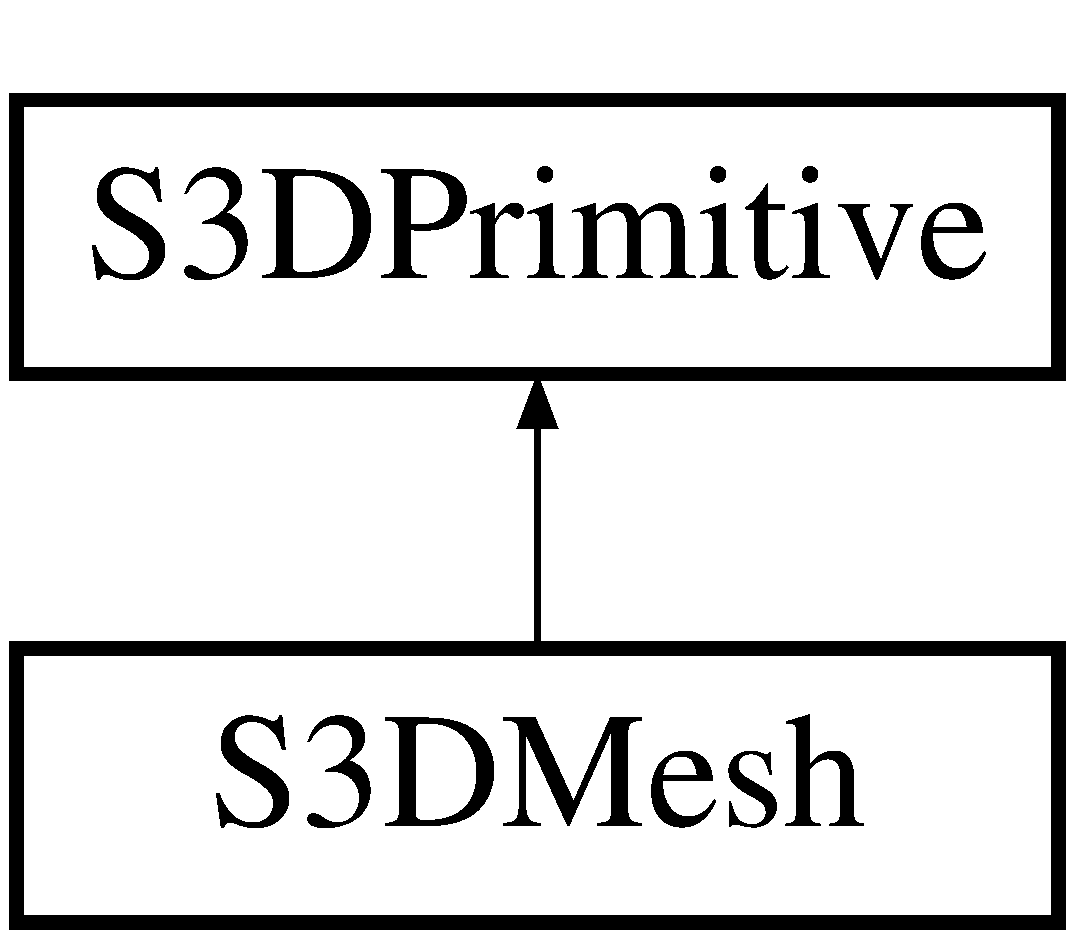
\includegraphics[height=2cm]{class_s3_d_mesh}
\end{center}
\end{figure}
\subsection*{Public Member Functions}
\begin{DoxyCompactItemize}
\item 
\hyperlink{class_s3_d_mesh_a810cf0f60312bc574e347d6248499258}{S3DMesh} (const char $\ast$file)
\begin{DoxyCompactList}\small\item\em Constructor for the Mesh, loads data from a file. \item\end{DoxyCompactList}\item 
void \hyperlink{class_s3_d_mesh_afc47824c491991604931f4ccb0520cd1}{draw} (S3DDevice $\ast$disp, S3DSurface window, S3DContext gc, \hyperlink{class_s3_d_z_buffer}{S3DZBuffer} $\ast$zbuffer)
\begin{DoxyCompactList}\small\item\em Draws the mesh. \item\end{DoxyCompactList}\item 
void \hyperlink{class_s3_d_mesh_a15edf10bf8a749627f11235c618734f7}{move} (double dx, double dy, double dz)
\begin{DoxyCompactList}\small\item\em Moves the mesh (translates it) relative to its coordinates. \item\end{DoxyCompactList}\item 
void \hyperlink{class_s3_d_mesh_ad1de35530a123dbb515e37afc8ecc0e3}{scale} (double fx, double fy, double fz)
\begin{DoxyCompactList}\small\item\em Scales the mesh. \item\end{DoxyCompactList}\item 
void \hyperlink{class_s3_d_mesh_affff1ac3ef33b293a9ec9881a4e13993}{rotate} (double rx, double ry, double rz, \hyperlink{class_s3_d_point}{S3DPoint} $\ast$anchor=NULL)
\begin{DoxyCompactList}\small\item\em Rotates the mesh around its center or another anchor point. \item\end{DoxyCompactList}\item 
double \hyperlink{class_s3_d_mesh_aa11c4dd0ce01443c07afaabc0e206881}{getZ} ()
\begin{DoxyCompactList}\small\item\em Returns the z-\/coordinate for the center of the mesh. \item\end{DoxyCompactList}\end{DoxyCompactItemize}


\subsection{Detailed Description}
This class is used to load a collection of triangles to use it as an entity. This class allows to load a collection of triangles from a file to get a complex entity. 

\subsection{Constructor \& Destructor Documentation}
\hypertarget{class_s3_d_mesh_a810cf0f60312bc574e347d6248499258}{
\index{S3DMesh@{S3DMesh}!S3DMesh@{S3DMesh}}
\index{S3DMesh@{S3DMesh}!S3DMesh@{S3DMesh}}
\subsubsection[{S3DMesh}]{\setlength{\rightskip}{0pt plus 5cm}S3DMesh::S3DMesh (const char $\ast$ {\em file})}}
\label{class_s3_d_mesh_a810cf0f60312bc574e347d6248499258}


Constructor for the Mesh, loads data from a file. 


\begin{DoxyParams}{Parameters}
\item[\mbox{$\leftarrow$} {\em file}]The filename of the file containing the data\end{DoxyParams}
Constructs a new instance of \hyperlink{class_s3_d_mesh}{S3DMesh} and loads data from a file to build a series of triangles, ready to be rendered on screen. 

\subsection{Member Function Documentation}
\hypertarget{class_s3_d_mesh_afc47824c491991604931f4ccb0520cd1}{
\index{S3DMesh@{S3DMesh}!draw@{draw}}
\index{draw@{draw}!S3DMesh@{S3DMesh}}
\subsubsection[{draw}]{\setlength{\rightskip}{0pt plus 5cm}void S3DMesh::draw (S3DDevice $\ast$ {\em disp}, \/  S3DSurface {\em window}, \/  S3DContext {\em gc}, \/  {\bf S3DZBuffer} $\ast$ {\em zbuffer})\hspace{0.3cm}{\ttfamily  \mbox{[}virtual\mbox{]}}}}
\label{class_s3_d_mesh_afc47824c491991604931f4ccb0520cd1}


Draws the mesh. 


\begin{DoxyParams}{Parameters}
\item[\mbox{$\leftarrow$} {\em disp}]The display device, the line will be drawn to \item[\mbox{$\leftarrow$} {\em window}]The surface, the line will be drawn to \item[\mbox{$\leftarrow$} {\em gc}]The context, the line will be drawn to \item[{\em zbuffer}]Pointer to the S3DZBuffer-\/Instance of the Simple3D-\/Instance.\end{DoxyParams}
Draws the mesh by drawing the triangles it consists of. This method does NOT contain platform-\/specific calls anymore, because it uses the underlying triangles to draw the mesh. The meaning and neccessity of disp, window and gc may vary between different platforms 

Implements \hyperlink{class_s3_d_primitive_a857f042bc63ae6233b63b60089e92b81}{S3DPrimitive}.

\hypertarget{class_s3_d_mesh_aa11c4dd0ce01443c07afaabc0e206881}{
\index{S3DMesh@{S3DMesh}!getZ@{getZ}}
\index{getZ@{getZ}!S3DMesh@{S3DMesh}}
\subsubsection[{getZ}]{\setlength{\rightskip}{0pt plus 5cm}double S3DMesh::getZ ()\hspace{0.3cm}{\ttfamily  \mbox{[}virtual\mbox{]}}}}
\label{class_s3_d_mesh_aa11c4dd0ce01443c07afaabc0e206881}


Returns the z-\/coordinate for the center of the mesh. 

This function is used for Z-\/Buffering and currently also for the painter's algorithm to determine the order in which the entities get drawn. 

Implements \hyperlink{class_s3_d_primitive_ab5b06d3a8e83216cc42554bb78afd2d9}{S3DPrimitive}.

\hypertarget{class_s3_d_mesh_a15edf10bf8a749627f11235c618734f7}{
\index{S3DMesh@{S3DMesh}!move@{move}}
\index{move@{move}!S3DMesh@{S3DMesh}}
\subsubsection[{move}]{\setlength{\rightskip}{0pt plus 5cm}void S3DMesh::move (double {\em dx}, \/  double {\em dy}, \/  double {\em dz})\hspace{0.3cm}{\ttfamily  \mbox{[}virtual\mbox{]}}}}
\label{class_s3_d_mesh_a15edf10bf8a749627f11235c618734f7}


Moves the mesh (translates it) relative to its coordinates. 


\begin{DoxyParams}{Parameters}
\item[\mbox{$\leftarrow$} {\em dx}]The distance the mesh is moved in x-\/direction \item[\mbox{$\leftarrow$} {\em dy}]The distance the mesh is moved in y-\/direction \item[\mbox{$\leftarrow$} {\em dz}]The distance the mesh is moved in z-\/direction \end{DoxyParams}


Implements \hyperlink{class_s3_d_primitive_a73a178ec2e1aa8e95f01baf0552724a9}{S3DPrimitive}.

\hypertarget{class_s3_d_mesh_affff1ac3ef33b293a9ec9881a4e13993}{
\index{S3DMesh@{S3DMesh}!rotate@{rotate}}
\index{rotate@{rotate}!S3DMesh@{S3DMesh}}
\subsubsection[{rotate}]{\setlength{\rightskip}{0pt plus 5cm}void S3DMesh::rotate (double {\em rx}, \/  double {\em ry}, \/  double {\em rz}, \/  {\bf S3DPoint} $\ast$ {\em anchor} = {\ttfamily NULL})\hspace{0.3cm}{\ttfamily  \mbox{[}virtual\mbox{]}}}}
\label{class_s3_d_mesh_affff1ac3ef33b293a9ec9881a4e13993}


Rotates the mesh around its center or another anchor point. 


\begin{DoxyParams}{Parameters}
\item[\mbox{$\leftarrow$} {\em rx}]The angle the mesh should be rotated around the x-\/axis \item[\mbox{$\leftarrow$} {\em ry}]The angle the mesh should be rotated around the y-\/axis \item[\mbox{$\leftarrow$} {\em rz}]The angle the mesh should be rotated around the z-\/axis \item[\mbox{$\leftarrow$} {\em anchor}]Optional. The point the mesh should be rotated around, instead of its own center.\end{DoxyParams}
This function allows to rotate the mesh around all three axis in any angle. If no anchor-\/point is passed, the mesh will be rotated around its own center, else it will rotate around the given point. 

Implements \hyperlink{class_s3_d_primitive_a23eb36b6bd48643e8f7be4b950592d9e}{S3DPrimitive}.

\hypertarget{class_s3_d_mesh_ad1de35530a123dbb515e37afc8ecc0e3}{
\index{S3DMesh@{S3DMesh}!scale@{scale}}
\index{scale@{scale}!S3DMesh@{S3DMesh}}
\subsubsection[{scale}]{\setlength{\rightskip}{0pt plus 5cm}void S3DMesh::scale (double {\em fx}, \/  double {\em fy}, \/  double {\em fz})}}
\label{class_s3_d_mesh_ad1de35530a123dbb515e37afc8ecc0e3}


Scales the mesh. 


\begin{DoxyParams}{Parameters}
\item[\mbox{$\leftarrow$} {\em fx}]Scaling factor along the x-\/axis \item[\mbox{$\leftarrow$} {\em fy}]Scaling factor along the y-\/axis \item[\mbox{$\leftarrow$} {\em fz}]Scaling factor along the z-\/axis\end{DoxyParams}
This method scales the mesh according to the given factors. Internal its also translated to preserve its center's coordinates. 

The documentation for this class was generated from the following files:\begin{DoxyCompactItemize}
\item 
\hyperlink{_s3_d_mesh_8h}{S3DMesh.h}\item 
\hyperlink{_s3_d_mesh_8cpp}{S3DMesh.cpp}\end{DoxyCompactItemize}

\hypertarget{class_s3_d_point}{
\section{S3DPoint Class Reference}
\label{class_s3_d_point}\index{S3DPoint@{S3DPoint}}
}


This class is used for representing 3d-\/coordinates.  




{\ttfamily \#include $<$S3DPoint.h$>$}

\subsection*{Public Member Functions}
\begin{DoxyCompactItemize}
\item 
\hyperlink{class_s3_d_point_adad5537c6692acccab628a6bc105d20e}{S3DPoint} ()
\begin{DoxyCompactList}\small\item\em Default constructor. \item\end{DoxyCompactList}\item 
\hyperlink{class_s3_d_point_ab03f0683b11340e8071eb8cdde1811b3}{S3DPoint} (double \hyperlink{class_s3_d_point_ae6b39611c603bd43ea67bcf4438a932a}{x}, double \hyperlink{class_s3_d_point_a487ab6dfdcb00ddbf9485f0b71ad7fb5}{y}, double \hyperlink{class_s3_d_point_ace7df3a87344170ddb4bfc92c3d5ec3d}{z})
\begin{DoxyCompactList}\small\item\em Mostly used constructor used for creating S3DPoints. \item\end{DoxyCompactList}\item 
void \hyperlink{class_s3_d_point_a18bbc742cbadc8d49d0600c3f80caf91}{move} (double dx, double dy, double dz)
\begin{DoxyCompactList}\small\item\em Moves the point (translates it) relative to its coordinates. \item\end{DoxyCompactList}\item 
void \hyperlink{class_s3_d_point_a59aee595c8ae9bfbb60915a09c06b0aa}{draw} (Display $\ast$d, Window w, GC g)
\begin{DoxyCompactList}\small\item\em Draws the point. \item\end{DoxyCompactList}\item 
void \hyperlink{class_s3_d_point_a4d51ed60f8d2e7ee2edd060cfdef22d4}{rotate} (double rx, double ry, double rz)
\item 
double \hyperlink{class_s3_d_point_a255a77e4ca340344be1b1bd6b6a3f418}{getZ} ()
\begin{DoxyCompactList}\small\item\em Returns the z-\/coordinate for the point. \item\end{DoxyCompactList}\end{DoxyCompactItemize}
\subsection*{Public Attributes}
\begin{DoxyCompactItemize}
\item 
double \hyperlink{class_s3_d_point_ae6b39611c603bd43ea67bcf4438a932a}{x}
\item 
double \hyperlink{class_s3_d_point_a487ab6dfdcb00ddbf9485f0b71ad7fb5}{y}
\item 
double \hyperlink{class_s3_d_point_ace7df3a87344170ddb4bfc92c3d5ec3d}{z}
\end{DoxyCompactItemize}


\subsection{Detailed Description}
This class is used for representing 3d-\/coordinates. This class is a representation of a point in 3D-\/space, thus a coordinate-\/triplet (x,y,z), that can be drawn though its not a primitive itself. 

\subsection{Constructor \& Destructor Documentation}
\hypertarget{class_s3_d_point_adad5537c6692acccab628a6bc105d20e}{
\index{S3DPoint@{S3DPoint}!S3DPoint@{S3DPoint}}
\index{S3DPoint@{S3DPoint}!S3DPoint@{S3DPoint}}
\subsubsection[{S3DPoint}]{\setlength{\rightskip}{0pt plus 5cm}S3DPoint::S3DPoint ()}}
\label{class_s3_d_point_adad5537c6692acccab628a6bc105d20e}


Default constructor. 

Creates a new instance of \hyperlink{class_s3_d_point}{S3DPoint} with coordinates (0,0,0), so the origin. \hypertarget{class_s3_d_point_ab03f0683b11340e8071eb8cdde1811b3}{
\index{S3DPoint@{S3DPoint}!S3DPoint@{S3DPoint}}
\index{S3DPoint@{S3DPoint}!S3DPoint@{S3DPoint}}
\subsubsection[{S3DPoint}]{\setlength{\rightskip}{0pt plus 5cm}S3DPoint::S3DPoint (double {\em px}, \/  double {\em py}, \/  double {\em pz})}}
\label{class_s3_d_point_ab03f0683b11340e8071eb8cdde1811b3}


Mostly used constructor used for creating S3DPoints. 


\begin{DoxyParams}{Parameters}
\item[\mbox{$\leftarrow$} {\em px}]X-\/Coordinate of the point \item[\mbox{$\leftarrow$} {\em py}]Y-\/Coordinate of the point \item[\mbox{$\leftarrow$} {\em pz}]Z-\/Coordinate of the point\end{DoxyParams}
Creates an new instance of a three-\/dimensional point with coordinates (x,y,z). Used in every primary to determine coordinates and used in projections. 

\subsection{Member Function Documentation}
\hypertarget{class_s3_d_point_a59aee595c8ae9bfbb60915a09c06b0aa}{
\index{S3DPoint@{S3DPoint}!draw@{draw}}
\index{draw@{draw}!S3DPoint@{S3DPoint}}
\subsubsection[{draw}]{\setlength{\rightskip}{0pt plus 5cm}void S3DPoint::draw (Display $\ast$ {\em d}, \/  Window {\em w}, \/  GC {\em g})}}
\label{class_s3_d_point_a59aee595c8ae9bfbb60915a09c06b0aa}


Draws the point. 


\begin{DoxyParams}{Parameters}
\item[\mbox{$\leftarrow$} {\em disp}]The display device, the line will be drawn to \item[\mbox{$\leftarrow$} {\em window}]The surface, the line will be drawn to \item[\mbox{$\leftarrow$} {\em gc}]The context, the line will be drawn to \item[{\em zbuffer}]Pointer to the S3DZBuffer-\/Instance of the Simple3D-\/Instance.\end{DoxyParams}
Draws the point using platform-\/dependent methods. The meaning and neccessity of disp, window and gc may vary between different platforms \hypertarget{class_s3_d_point_a255a77e4ca340344be1b1bd6b6a3f418}{
\index{S3DPoint@{S3DPoint}!getZ@{getZ}}
\index{getZ@{getZ}!S3DPoint@{S3DPoint}}
\subsubsection[{getZ}]{\setlength{\rightskip}{0pt plus 5cm}double S3DPoint::getZ ()}}
\label{class_s3_d_point_a255a77e4ca340344be1b1bd6b6a3f418}


Returns the z-\/coordinate for the point. 

This function is used for Z-\/Buffering and currently also for the painter's algorithm to determine the order in which the entities get drawn. \hypertarget{class_s3_d_point_a18bbc742cbadc8d49d0600c3f80caf91}{
\index{S3DPoint@{S3DPoint}!move@{move}}
\index{move@{move}!S3DPoint@{S3DPoint}}
\subsubsection[{move}]{\setlength{\rightskip}{0pt plus 5cm}void S3DPoint::move (double {\em dx}, \/  double {\em dy}, \/  double {\em dz})}}
\label{class_s3_d_point_a18bbc742cbadc8d49d0600c3f80caf91}


Moves the point (translates it) relative to its coordinates. 


\begin{DoxyParams}{Parameters}
\item[\mbox{$\leftarrow$} {\em dx}]The distance the point is moved in x-\/direction \item[\mbox{$\leftarrow$} {\em dy}]The distance the point is moved in y-\/direction \item[\mbox{$\leftarrow$} {\em dz}]The distance the point is moved in z-\/direction \end{DoxyParams}
\hypertarget{class_s3_d_point_a4d51ed60f8d2e7ee2edd060cfdef22d4}{
\index{S3DPoint@{S3DPoint}!rotate@{rotate}}
\index{rotate@{rotate}!S3DPoint@{S3DPoint}}
\subsubsection[{rotate}]{\setlength{\rightskip}{0pt plus 5cm}void S3DPoint::rotate (double {\em rx}, \/  double {\em ry}, \/  double {\em rz})\hspace{0.3cm}{\ttfamily  \mbox{[}inline\mbox{]}}}}
\label{class_s3_d_point_a4d51ed60f8d2e7ee2edd060cfdef22d4}


\subsection{Member Data Documentation}
\hypertarget{class_s3_d_point_ae6b39611c603bd43ea67bcf4438a932a}{
\index{S3DPoint@{S3DPoint}!x@{x}}
\index{x@{x}!S3DPoint@{S3DPoint}}
\subsubsection[{x}]{\setlength{\rightskip}{0pt plus 5cm}double {\bf S3DPoint::x}}}
\label{class_s3_d_point_ae6b39611c603bd43ea67bcf4438a932a}
\hypertarget{class_s3_d_point_a487ab6dfdcb00ddbf9485f0b71ad7fb5}{
\index{S3DPoint@{S3DPoint}!y@{y}}
\index{y@{y}!S3DPoint@{S3DPoint}}
\subsubsection[{y}]{\setlength{\rightskip}{0pt plus 5cm}double {\bf S3DPoint::y}}}
\label{class_s3_d_point_a487ab6dfdcb00ddbf9485f0b71ad7fb5}
\hypertarget{class_s3_d_point_ace7df3a87344170ddb4bfc92c3d5ec3d}{
\index{S3DPoint@{S3DPoint}!z@{z}}
\index{z@{z}!S3DPoint@{S3DPoint}}
\subsubsection[{z}]{\setlength{\rightskip}{0pt plus 5cm}double {\bf S3DPoint::z}}}
\label{class_s3_d_point_ace7df3a87344170ddb4bfc92c3d5ec3d}


The documentation for this class was generated from the following files:\begin{DoxyCompactItemize}
\item 
\hyperlink{_s3_d_point_8h}{S3DPoint.h}\item 
\hyperlink{_s3_d_point_8cpp}{S3DPoint.cpp}\end{DoxyCompactItemize}

\hypertarget{class_s3_d_primitive}{
\section{S3DPrimitive Class Reference}
\label{class_s3_d_primitive}\index{S3DPrimitive@{S3DPrimitive}}
}


This class is the base of all primitives in S3D.  




{\ttfamily \#include $<$S3DPrimitive.h$>$}

Inheritance diagram for S3DPrimitive:\begin{figure}[H]
\begin{center}
\leavevmode
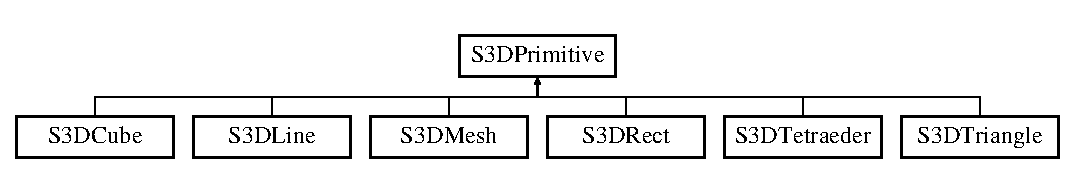
\includegraphics[height=1.88552cm]{class_s3_d_primitive}
\end{center}
\end{figure}
\subsection*{Public Member Functions}
\begin{DoxyCompactItemize}
\item 
virtual void \hyperlink{class_s3_d_primitive_a857f042bc63ae6233b63b60089e92b81}{draw} (\hyperlink{types_8h_a25c0773a29204332721bde1b164d0b84}{S3DDevice} $\ast$disp, \hyperlink{types_8h_a4afc89c514af26434688c7e8b382ba5e}{S3DSurface} window, \hyperlink{types_8h_a46f30693e0040340e595d8228cc31779}{S3DContext} gc, \hyperlink{class_s3_d_z_buffer}{S3DZBuffer} $\ast$zbuffer)=0
\begin{DoxyCompactList}\small\item\em Virtual method. Implementations are responsible for drawing the primitive. \item\end{DoxyCompactList}\item 
virtual void \hyperlink{class_s3_d_primitive_a23eb36b6bd48643e8f7be4b950592d9e}{rotate} (double rx, double ry, double rz, \hyperlink{class_s3_d_point}{S3DPoint} $\ast$anchor=NULL)=0
\begin{DoxyCompactList}\small\item\em Virtual method. Implementations are responsible for rotating the primitive. \item\end{DoxyCompactList}\item 
virtual void \hyperlink{class_s3_d_primitive_a73a178ec2e1aa8e95f01baf0552724a9}{move} (double dx, double dy, double dz)=0
\begin{DoxyCompactList}\small\item\em Virtual method. Implementations are responsible for moving the primitive. \item\end{DoxyCompactList}\item 
virtual double \hyperlink{class_s3_d_primitive_ab5b06d3a8e83216cc42554bb78afd2d9}{getZ} ()=0
\begin{DoxyCompactList}\small\item\em Virtual method. Implementations are responsible for return some z-\/Value the primitive. \item\end{DoxyCompactList}\item 
bool \hyperlink{class_s3_d_primitive_a36948fee7526b4c0634d16372ebb3e56}{getFillMode} ()
\begin{DoxyCompactList}\small\item\em Returns if the primitive is filled or just wireframe. \item\end{DoxyCompactList}\item 
void \hyperlink{class_s3_d_primitive_afd54077b1dbe256b9c6dfe67da7b0a0b}{setFillMode} (bool fill)
\begin{DoxyCompactList}\small\item\em Used to influence, if the primitive is filled or just wireframe. \item\end{DoxyCompactList}\item 
unsigned long \hyperlink{class_s3_d_primitive_a4102845e7754e44c51a87c0fcb391c73}{getColor} ()
\begin{DoxyCompactList}\small\item\em Returns the color of the primitive. \item\end{DoxyCompactList}\item 
void \hyperlink{class_s3_d_primitive_a1c8f036193987522bdfb6a49b9b74000}{setColor} (unsigned long c)
\begin{DoxyCompactList}\small\item\em Sets the color of the primitive. \item\end{DoxyCompactList}\end{DoxyCompactItemize}
\subsection*{Public Attributes}
\begin{DoxyCompactItemize}
\item 
unsigned int \hyperlink{class_s3_d_primitive_ae8ff735495c481dbbd0c99ffe16d954f}{id}
\end{DoxyCompactItemize}
\subsection*{Static Public Attributes}
\begin{DoxyCompactItemize}
\item 
static unsigned int \hyperlink{class_s3_d_primitive_a08ee26517002051f19202d8b62bf2b46}{id\_\-max} = 1
\end{DoxyCompactItemize}
\subsection*{Protected Attributes}
\begin{DoxyCompactItemize}
\item 
bool \hyperlink{class_s3_d_primitive_ae5b091719cc1afa825a4ba0e1dfce670}{isFilled}
\item 
unsigned long \hyperlink{class_s3_d_primitive_afc81699d5253aab2757a2c5e33848a22}{color}
\end{DoxyCompactItemize}


\subsection{Detailed Description}
This class is the base of all primitives in S3D. This class is the base-\/class for ALL primitives in S3D. It contains the virtual methods, derived primitives need to implement. Its the main interface for primitives. 

\subsection{Member Function Documentation}
\hypertarget{class_s3_d_primitive_a857f042bc63ae6233b63b60089e92b81}{
\index{S3DPrimitive@{S3DPrimitive}!draw@{draw}}
\index{draw@{draw}!S3DPrimitive@{S3DPrimitive}}
\subsubsection[{draw}]{\setlength{\rightskip}{0pt plus 5cm}virtual void S3DPrimitive::draw ({\bf S3DDevice} $\ast$ {\em disp}, \/  {\bf S3DSurface} {\em window}, \/  {\bf S3DContext} {\em gc}, \/  {\bf S3DZBuffer} $\ast$ {\em zbuffer})\hspace{0.3cm}{\ttfamily  \mbox{[}pure virtual\mbox{]}}}}
\label{class_s3_d_primitive_a857f042bc63ae6233b63b60089e92b81}


Virtual method. Implementations are responsible for drawing the primitive. 



Implemented in \hyperlink{class_s3_d_line_aa7732c2d83fecb5d9934863d0e7875c1}{S3DLine}, \hyperlink{class_s3_d_mesh_afc47824c491991604931f4ccb0520cd1}{S3DMesh}, and \hyperlink{class_s3_d_triangle_acf6924908c89d6bbc5af23769243beaf}{S3DTriangle}.

\hypertarget{class_s3_d_primitive_a4102845e7754e44c51a87c0fcb391c73}{
\index{S3DPrimitive@{S3DPrimitive}!getColor@{getColor}}
\index{getColor@{getColor}!S3DPrimitive@{S3DPrimitive}}
\subsubsection[{getColor}]{\setlength{\rightskip}{0pt plus 5cm}unsigned long S3DPrimitive::getColor ()}}
\label{class_s3_d_primitive_a4102845e7754e44c51a87c0fcb391c73}


Returns the color of the primitive. 



Reimplemented in \hyperlink{class_s3_d_cube_ab856b6fa4c1b72be7d2d7b79e26f3c38}{S3DCube}, \hyperlink{class_s3_d_line_a62b49873ae3356cf997ca1fd87a1b7de}{S3DLine}, \hyperlink{class_s3_d_rect_adbf17caac29e632afb9f380e3821a256}{S3DRect}, \hyperlink{class_s3_d_tetraeder_ab79d98573d008f21c9a77f9d3633d6ae}{S3DTetraeder}, and \hyperlink{class_s3_d_triangle_ade8ba96094206ee3dff5c3bc743e0a1c}{S3DTriangle}.

\hypertarget{class_s3_d_primitive_a36948fee7526b4c0634d16372ebb3e56}{
\index{S3DPrimitive@{S3DPrimitive}!getFillMode@{getFillMode}}
\index{getFillMode@{getFillMode}!S3DPrimitive@{S3DPrimitive}}
\subsubsection[{getFillMode}]{\setlength{\rightskip}{0pt plus 5cm}bool S3DPrimitive::getFillMode ()}}
\label{class_s3_d_primitive_a36948fee7526b4c0634d16372ebb3e56}


Returns if the primitive is filled or just wireframe. 

\hypertarget{class_s3_d_primitive_ab5b06d3a8e83216cc42554bb78afd2d9}{
\index{S3DPrimitive@{S3DPrimitive}!getZ@{getZ}}
\index{getZ@{getZ}!S3DPrimitive@{S3DPrimitive}}
\subsubsection[{getZ}]{\setlength{\rightskip}{0pt plus 5cm}virtual double S3DPrimitive::getZ ()\hspace{0.3cm}{\ttfamily  \mbox{[}pure virtual\mbox{]}}}}
\label{class_s3_d_primitive_ab5b06d3a8e83216cc42554bb78afd2d9}


Virtual method. Implementations are responsible for return some z-\/Value the primitive. 



Implemented in \hyperlink{class_s3_d_cube_a4ac1d080b330d6b69d24097f746ddd4c}{S3DCube}, \hyperlink{class_s3_d_line_a72aabdbb4d3d0c3ea36f5fda7b059f6a}{S3DLine}, \hyperlink{class_s3_d_mesh_aa11c4dd0ce01443c07afaabc0e206881}{S3DMesh}, \hyperlink{class_s3_d_rect_a7b3fb925a55d8a22a354829d6a5afa3d}{S3DRect}, \hyperlink{class_s3_d_tetraeder_a5f77481efa810aafb63e9d1d5c14ceea}{S3DTetraeder}, and \hyperlink{class_s3_d_triangle_a35428b5799c8d51a6c57d1fdb5b575a1}{S3DTriangle}.

\hypertarget{class_s3_d_primitive_a73a178ec2e1aa8e95f01baf0552724a9}{
\index{S3DPrimitive@{S3DPrimitive}!move@{move}}
\index{move@{move}!S3DPrimitive@{S3DPrimitive}}
\subsubsection[{move}]{\setlength{\rightskip}{0pt plus 5cm}virtual void S3DPrimitive::move (double {\em dx}, \/  double {\em dy}, \/  double {\em dz})\hspace{0.3cm}{\ttfamily  \mbox{[}pure virtual\mbox{]}}}}
\label{class_s3_d_primitive_a73a178ec2e1aa8e95f01baf0552724a9}


Virtual method. Implementations are responsible for moving the primitive. 



Implemented in \hyperlink{class_s3_d_cube_ab21a1988528297602452984f8a3c093e}{S3DCube}, \hyperlink{class_s3_d_line_a38203e499c32f14ff5da3b7c17861881}{S3DLine}, \hyperlink{class_s3_d_mesh_a15edf10bf8a749627f11235c618734f7}{S3DMesh}, \hyperlink{class_s3_d_rect_a97fcf9a2380d07c59bc12db8bd5949bc}{S3DRect}, \hyperlink{class_s3_d_tetraeder_a3acda1d545e2f078abf299b1c424b7bc}{S3DTetraeder}, and \hyperlink{class_s3_d_triangle_a7f168122e4ed627fcb6489852a56982b}{S3DTriangle}.

\hypertarget{class_s3_d_primitive_a23eb36b6bd48643e8f7be4b950592d9e}{
\index{S3DPrimitive@{S3DPrimitive}!rotate@{rotate}}
\index{rotate@{rotate}!S3DPrimitive@{S3DPrimitive}}
\subsubsection[{rotate}]{\setlength{\rightskip}{0pt plus 5cm}virtual void S3DPrimitive::rotate (double {\em rx}, \/  double {\em ry}, \/  double {\em rz}, \/  {\bf S3DPoint} $\ast$ {\em anchor} = {\ttfamily NULL})\hspace{0.3cm}{\ttfamily  \mbox{[}pure virtual\mbox{]}}}}
\label{class_s3_d_primitive_a23eb36b6bd48643e8f7be4b950592d9e}


Virtual method. Implementations are responsible for rotating the primitive. 



Implemented in \hyperlink{class_s3_d_cube_a2e574649ca6ddd805c5ecdb7932f3ac1}{S3DCube}, \hyperlink{class_s3_d_line_a4d23495df2c8f45855d8b80d30b01d30}{S3DLine}, \hyperlink{class_s3_d_mesh_affff1ac3ef33b293a9ec9881a4e13993}{S3DMesh}, \hyperlink{class_s3_d_rect_a1d3b8406b588abf19cff5f8a6d6de2e2}{S3DRect}, \hyperlink{class_s3_d_tetraeder_aa06cc6b851e9a3abce9f68830340007a}{S3DTetraeder}, and \hyperlink{class_s3_d_triangle_a3e739f6c9c176e58cb734db7328cf039}{S3DTriangle}.

\hypertarget{class_s3_d_primitive_a1c8f036193987522bdfb6a49b9b74000}{
\index{S3DPrimitive@{S3DPrimitive}!setColor@{setColor}}
\index{setColor@{setColor}!S3DPrimitive@{S3DPrimitive}}
\subsubsection[{setColor}]{\setlength{\rightskip}{0pt plus 5cm}void S3DPrimitive::setColor (unsigned long {\em c})}}
\label{class_s3_d_primitive_a1c8f036193987522bdfb6a49b9b74000}


Sets the color of the primitive. 


\begin{DoxyParams}{Parameters}
\item[\mbox{$\leftarrow$} {\em c}]The color as unsigned long (as produced by RGB-\/macro), the primitive will get. \end{DoxyParams}


Reimplemented in \hyperlink{class_s3_d_cube_a9c48875a16cc0ace3a3092e98663b785}{S3DCube}, \hyperlink{class_s3_d_line_a9feaf056477e858a7b0248a7b5cdd222}{S3DLine}, \hyperlink{class_s3_d_rect_af1a976fbe476e7096b2ceded7ab1659c}{S3DRect}, \hyperlink{class_s3_d_tetraeder_a99856377365e5c26c1f86155909725ed}{S3DTetraeder}, and \hyperlink{class_s3_d_triangle_a2c60503c3bae194ec8247a0e2467c915}{S3DTriangle}.

\hypertarget{class_s3_d_primitive_afd54077b1dbe256b9c6dfe67da7b0a0b}{
\index{S3DPrimitive@{S3DPrimitive}!setFillMode@{setFillMode}}
\index{setFillMode@{setFillMode}!S3DPrimitive@{S3DPrimitive}}
\subsubsection[{setFillMode}]{\setlength{\rightskip}{0pt plus 5cm}void S3DPrimitive::setFillMode (bool {\em fill})}}
\label{class_s3_d_primitive_afd54077b1dbe256b9c6dfe67da7b0a0b}


Used to influence, if the primitive is filled or just wireframe. 


\begin{DoxyParams}{Parameters}
\item[\mbox{$\leftarrow$} {\em fill}]True, to make the primitive filled, else false. \end{DoxyParams}


\subsection{Member Data Documentation}
\hypertarget{class_s3_d_primitive_afc81699d5253aab2757a2c5e33848a22}{
\index{S3DPrimitive@{S3DPrimitive}!color@{color}}
\index{color@{color}!S3DPrimitive@{S3DPrimitive}}
\subsubsection[{color}]{\setlength{\rightskip}{0pt plus 5cm}unsigned long {\bf S3DPrimitive::color}\hspace{0.3cm}{\ttfamily  \mbox{[}protected\mbox{]}}}}
\label{class_s3_d_primitive_afc81699d5253aab2757a2c5e33848a22}
\hypertarget{class_s3_d_primitive_ae8ff735495c481dbbd0c99ffe16d954f}{
\index{S3DPrimitive@{S3DPrimitive}!id@{id}}
\index{id@{id}!S3DPrimitive@{S3DPrimitive}}
\subsubsection[{id}]{\setlength{\rightskip}{0pt plus 5cm}unsigned int {\bf S3DPrimitive::id}}}
\label{class_s3_d_primitive_ae8ff735495c481dbbd0c99ffe16d954f}
\hypertarget{class_s3_d_primitive_a08ee26517002051f19202d8b62bf2b46}{
\index{S3DPrimitive@{S3DPrimitive}!id\_\-max@{id\_\-max}}
\index{id\_\-max@{id\_\-max}!S3DPrimitive@{S3DPrimitive}}
\subsubsection[{id\_\-max}]{\setlength{\rightskip}{0pt plus 5cm}unsigned int {\bf S3DPrimitive::id\_\-max} = 1\hspace{0.3cm}{\ttfamily  \mbox{[}static\mbox{]}}}}
\label{class_s3_d_primitive_a08ee26517002051f19202d8b62bf2b46}
\hypertarget{class_s3_d_primitive_ae5b091719cc1afa825a4ba0e1dfce670}{
\index{S3DPrimitive@{S3DPrimitive}!isFilled@{isFilled}}
\index{isFilled@{isFilled}!S3DPrimitive@{S3DPrimitive}}
\subsubsection[{isFilled}]{\setlength{\rightskip}{0pt plus 5cm}bool {\bf S3DPrimitive::isFilled}\hspace{0.3cm}{\ttfamily  \mbox{[}protected\mbox{]}}}}
\label{class_s3_d_primitive_ae5b091719cc1afa825a4ba0e1dfce670}


The documentation for this class was generated from the following files:\begin{DoxyCompactItemize}
\item 
\hyperlink{_s3_d_primitive_8h}{S3DPrimitive.h}\item 
\hyperlink{_s3_d_primitive_8cpp}{S3DPrimitive.cpp}\end{DoxyCompactItemize}

\hypertarget{class_s3_d_rect}{
\section{S3DRect Class Reference}
\label{class_s3_d_rect}\index{S3DRect@{S3DRect}}
}
Inheritance diagram for S3DRect:\begin{figure}[H]
\begin{center}
\leavevmode
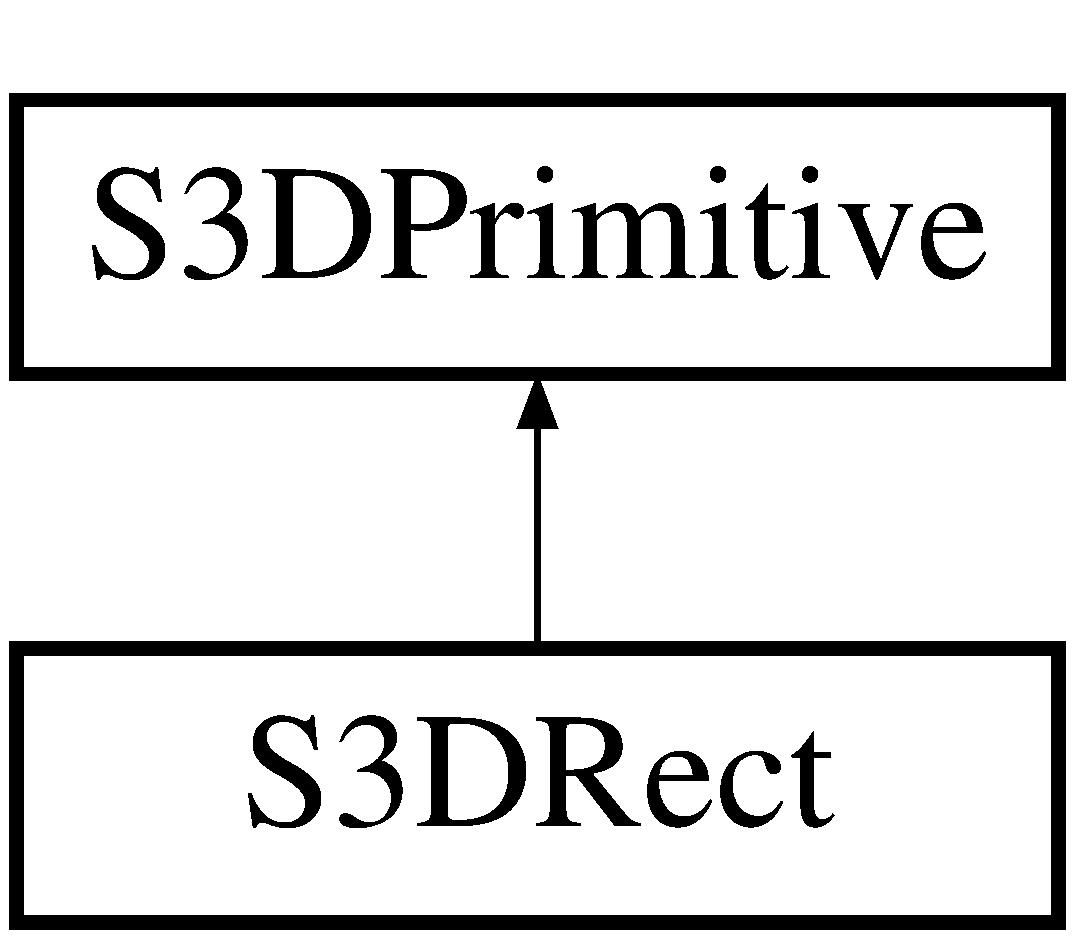
\includegraphics[height=2cm]{class_s3_d_rect}
\end{center}
\end{figure}
\subsection*{Public Member Functions}
\begin{DoxyCompactItemize}
\item 
\hypertarget{class_s3_d_rect_a30160c448c675829ced3c254a01ccb6e}{
{\bfseries S3DRect} (\hyperlink{class_s3_d_point}{S3DPoint} points\mbox{[}4\mbox{]})}
\label{class_s3_d_rect_a30160c448c675829ced3c254a01ccb6e}

\item 
\hypertarget{class_s3_d_rect_adfec4ab2501bd4cfef0f5fd82d769942}{
{\bfseries S3DRect} (\hyperlink{class_s3_d_point}{S3DPoint} a, \hyperlink{class_s3_d_point}{S3DPoint} b, \hyperlink{class_s3_d_point}{S3DPoint} c, \hyperlink{class_s3_d_point}{S3DPoint} d)}
\label{class_s3_d_rect_adfec4ab2501bd4cfef0f5fd82d769942}

\item 
\hypertarget{class_s3_d_rect_a97fcf9a2380d07c59bc12db8bd5949bc}{
void \hyperlink{class_s3_d_rect_a97fcf9a2380d07c59bc12db8bd5949bc}{move} (double dx, double dy, double dz)}
\label{class_s3_d_rect_a97fcf9a2380d07c59bc12db8bd5949bc}

\begin{DoxyCompactList}\small\item\em Virtual method. Implementations are responsible for moving the primitive. \item\end{DoxyCompactList}\item 
\hypertarget{class_s3_d_rect_a1d3b8406b588abf19cff5f8a6d6de2e2}{
void \hyperlink{class_s3_d_rect_a1d3b8406b588abf19cff5f8a6d6de2e2}{rotate} (double rx, double ry, double rz, \hyperlink{class_s3_d_point}{S3DPoint} $\ast$anchor=NULL)}
\label{class_s3_d_rect_a1d3b8406b588abf19cff5f8a6d6de2e2}

\begin{DoxyCompactList}\small\item\em Virtual method. Implementations are responsible for rotating the primitive. \item\end{DoxyCompactList}\item 
\hypertarget{class_s3_d_rect_adfa6596cc2a62c83709f0f3a040333c1}{
void {\bfseries draw} (S3DDevice $\ast$d, S3DSurface w, S3DContext g)}
\label{class_s3_d_rect_adfa6596cc2a62c83709f0f3a040333c1}

\item 
void \hyperlink{class_s3_d_rect_af1a976fbe476e7096b2ceded7ab1659c}{setColor} (unsigned long c)
\begin{DoxyCompactList}\small\item\em Sets the color of the primitive. \item\end{DoxyCompactList}\item 
\hypertarget{class_s3_d_rect_adbf17caac29e632afb9f380e3821a256}{
unsigned long \hyperlink{class_s3_d_rect_adbf17caac29e632afb9f380e3821a256}{getColor} ()}
\label{class_s3_d_rect_adbf17caac29e632afb9f380e3821a256}

\begin{DoxyCompactList}\small\item\em Returns the color of the primitive. \item\end{DoxyCompactList}\item 
\hypertarget{class_s3_d_rect_a626b39ee85c2ab329258bba6ee0ac255}{
\hyperlink{class_s3_d_point}{S3DPoint} $\ast$ {\bfseries getPoints} ()}
\label{class_s3_d_rect_a626b39ee85c2ab329258bba6ee0ac255}

\item 
\hypertarget{class_s3_d_rect_a7b3fb925a55d8a22a354829d6a5afa3d}{
double \hyperlink{class_s3_d_rect_a7b3fb925a55d8a22a354829d6a5afa3d}{getZ} ()}
\label{class_s3_d_rect_a7b3fb925a55d8a22a354829d6a5afa3d}

\begin{DoxyCompactList}\small\item\em Virtual method. Implementations are responsible for return some z-\/Value the primitive. \item\end{DoxyCompactList}\end{DoxyCompactItemize}


\subsection{Member Function Documentation}
\hypertarget{class_s3_d_rect_af1a976fbe476e7096b2ceded7ab1659c}{
\index{S3DRect@{S3DRect}!setColor@{setColor}}
\index{setColor@{setColor}!S3DRect@{S3DRect}}
\subsubsection[{setColor}]{\setlength{\rightskip}{0pt plus 5cm}void S3DRect::setColor (unsigned long {\em c})}}
\label{class_s3_d_rect_af1a976fbe476e7096b2ceded7ab1659c}


Sets the color of the primitive. 


\begin{DoxyParams}{Parameters}
\item[\mbox{$\leftarrow$} {\em c}]The color as unsigned long (as produced by RGB-\/macro), the primitive will get. \end{DoxyParams}


Reimplemented from \hyperlink{class_s3_d_primitive_a1c8f036193987522bdfb6a49b9b74000}{S3DPrimitive}.



The documentation for this class was generated from the following files:\begin{DoxyCompactItemize}
\item 
Simple3D/S3DRect.h\item 
Simple3D/S3DRect.cpp\end{DoxyCompactItemize}

\hypertarget{class_s3_d_tetraeder}{
\section{S3DTetraeder Class Reference}
\label{class_s3_d_tetraeder}\index{S3DTetraeder@{S3DTetraeder}}
}


{\ttfamily \#include $<$S3DTetraeder.h$>$}

Inheritance diagram for S3DTetraeder:\begin{figure}[H]
\begin{center}
\leavevmode
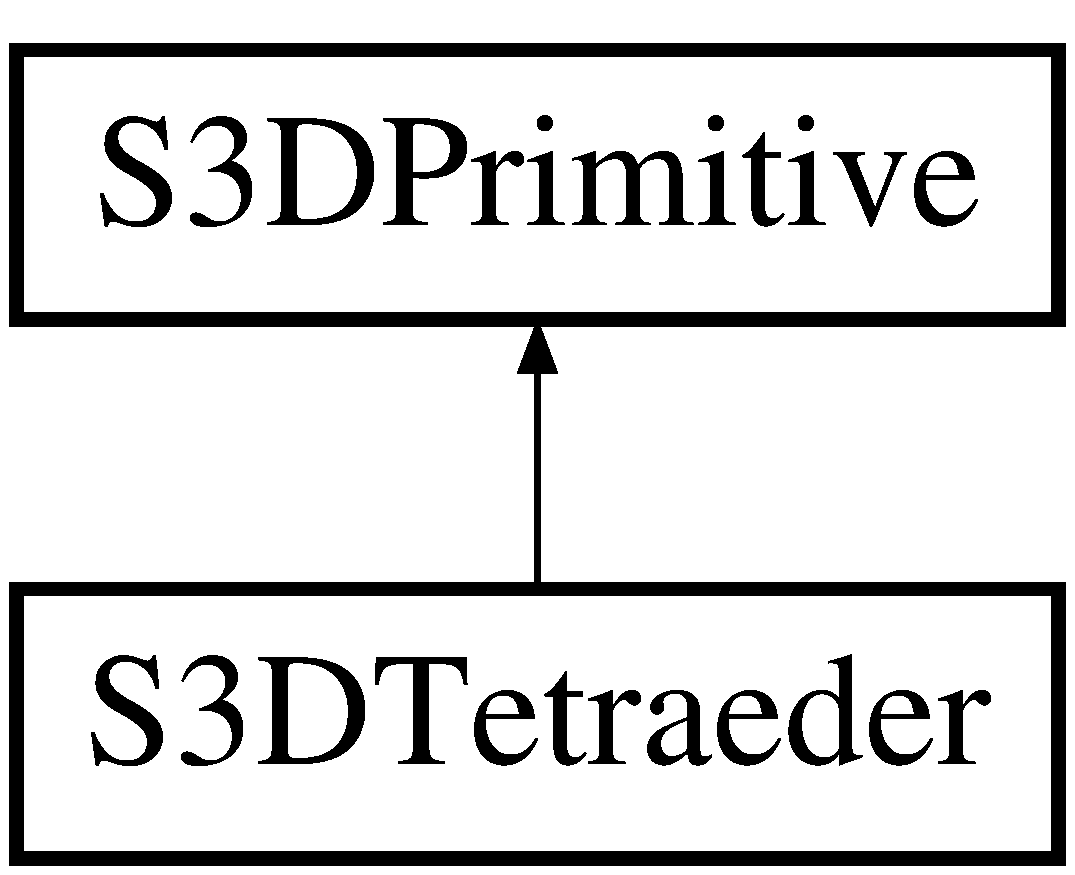
\includegraphics[height=2cm]{class_s3_d_tetraeder}
\end{center}
\end{figure}
\subsection*{Public Member Functions}
\begin{DoxyCompactItemize}
\item 
\hyperlink{class_s3_d_tetraeder_ac70078c42e24160a8759fafff847ee30}{S3DTetraeder} (\hyperlink{class_s3_d_point}{S3DPoint} points\mbox{[}4\mbox{]})
\item 
\hyperlink{class_s3_d_tetraeder_a98dc7f23bd82419321b7a086159e25d3}{S3DTetraeder} (\hyperlink{class_s3_d_point}{S3DPoint} a, \hyperlink{class_s3_d_point}{S3DPoint} b, \hyperlink{class_s3_d_point}{S3DPoint} c, \hyperlink{class_s3_d_point}{S3DPoint} d)
\item 
void \hyperlink{class_s3_d_tetraeder_a3acda1d545e2f078abf299b1c424b7bc}{move} (double dx, double dy, double dz)
\begin{DoxyCompactList}\small\item\em Virtual method. Implementations are responsible for moving the primitive. \item\end{DoxyCompactList}\item 
void \hyperlink{class_s3_d_tetraeder_aa06cc6b851e9a3abce9f68830340007a}{rotate} (double rx, double ry, double rz, \hyperlink{class_s3_d_point}{S3DPoint} $\ast$anchor=NULL)
\begin{DoxyCompactList}\small\item\em Virtual method. Implementations are responsible for rotating the primitive. \item\end{DoxyCompactList}\item 
void \hyperlink{class_s3_d_tetraeder_a35594d3c61c89fa1dbe7a6a115cea56b}{draw} (\hyperlink{types_8h_a25c0773a29204332721bde1b164d0b84}{S3DDevice} $\ast$d, \hyperlink{types_8h_a4afc89c514af26434688c7e8b382ba5e}{S3DSurface} w, \hyperlink{types_8h_a46f30693e0040340e595d8228cc31779}{S3DContext} g)
\item 
void \hyperlink{class_s3_d_tetraeder_a99856377365e5c26c1f86155909725ed}{setColor} (unsigned long c)
\begin{DoxyCompactList}\small\item\em Sets the color of the primitive. \item\end{DoxyCompactList}\item 
unsigned long \hyperlink{class_s3_d_tetraeder_ab79d98573d008f21c9a77f9d3633d6ae}{getColor} ()
\begin{DoxyCompactList}\small\item\em Returns the color of the primitive. \item\end{DoxyCompactList}\item 
\hyperlink{class_s3_d_point}{S3DPoint} $\ast$ \hyperlink{class_s3_d_tetraeder_a2be4bd418fda569bf8bbfc0fbd70ef1b}{getPoints} ()
\item 
double \hyperlink{class_s3_d_tetraeder_a5f77481efa810aafb63e9d1d5c14ceea}{getZ} ()
\begin{DoxyCompactList}\small\item\em Virtual method. Implementations are responsible for return some z-\/Value the primitive. \item\end{DoxyCompactList}\end{DoxyCompactItemize}


\subsection{Constructor \& Destructor Documentation}
\hypertarget{class_s3_d_tetraeder_ac70078c42e24160a8759fafff847ee30}{
\index{S3DTetraeder@{S3DTetraeder}!S3DTetraeder@{S3DTetraeder}}
\index{S3DTetraeder@{S3DTetraeder}!S3DTetraeder@{S3DTetraeder}}
\subsubsection[{S3DTetraeder}]{\setlength{\rightskip}{0pt plus 5cm}S3DTetraeder::S3DTetraeder ({\bf S3DPoint} {\em points}\mbox{[}4\mbox{]})}}
\label{class_s3_d_tetraeder_ac70078c42e24160a8759fafff847ee30}
\hypertarget{class_s3_d_tetraeder_a98dc7f23bd82419321b7a086159e25d3}{
\index{S3DTetraeder@{S3DTetraeder}!S3DTetraeder@{S3DTetraeder}}
\index{S3DTetraeder@{S3DTetraeder}!S3DTetraeder@{S3DTetraeder}}
\subsubsection[{S3DTetraeder}]{\setlength{\rightskip}{0pt plus 5cm}S3DTetraeder::S3DTetraeder ({\bf S3DPoint} {\em a}, \/  {\bf S3DPoint} {\em b}, \/  {\bf S3DPoint} {\em c}, \/  {\bf S3DPoint} {\em d})}}
\label{class_s3_d_tetraeder_a98dc7f23bd82419321b7a086159e25d3}


\subsection{Member Function Documentation}
\hypertarget{class_s3_d_tetraeder_a35594d3c61c89fa1dbe7a6a115cea56b}{
\index{S3DTetraeder@{S3DTetraeder}!draw@{draw}}
\index{draw@{draw}!S3DTetraeder@{S3DTetraeder}}
\subsubsection[{draw}]{\setlength{\rightskip}{0pt plus 5cm}void S3DTetraeder::draw ({\bf S3DDevice} $\ast$ {\em d}, \/  {\bf S3DSurface} {\em w}, \/  {\bf S3DContext} {\em g})}}
\label{class_s3_d_tetraeder_a35594d3c61c89fa1dbe7a6a115cea56b}
\hypertarget{class_s3_d_tetraeder_ab79d98573d008f21c9a77f9d3633d6ae}{
\index{S3DTetraeder@{S3DTetraeder}!getColor@{getColor}}
\index{getColor@{getColor}!S3DTetraeder@{S3DTetraeder}}
\subsubsection[{getColor}]{\setlength{\rightskip}{0pt plus 5cm}unsigned long S3DTetraeder::getColor ()}}
\label{class_s3_d_tetraeder_ab79d98573d008f21c9a77f9d3633d6ae}


Returns the color of the primitive. 



Reimplemented from \hyperlink{class_s3_d_primitive_a4102845e7754e44c51a87c0fcb391c73}{S3DPrimitive}.

\hypertarget{class_s3_d_tetraeder_a2be4bd418fda569bf8bbfc0fbd70ef1b}{
\index{S3DTetraeder@{S3DTetraeder}!getPoints@{getPoints}}
\index{getPoints@{getPoints}!S3DTetraeder@{S3DTetraeder}}
\subsubsection[{getPoints}]{\setlength{\rightskip}{0pt plus 5cm}{\bf S3DPoint} $\ast$ S3DTetraeder::getPoints ()}}
\label{class_s3_d_tetraeder_a2be4bd418fda569bf8bbfc0fbd70ef1b}
\hypertarget{class_s3_d_tetraeder_a5f77481efa810aafb63e9d1d5c14ceea}{
\index{S3DTetraeder@{S3DTetraeder}!getZ@{getZ}}
\index{getZ@{getZ}!S3DTetraeder@{S3DTetraeder}}
\subsubsection[{getZ}]{\setlength{\rightskip}{0pt plus 5cm}double S3DTetraeder::getZ ()\hspace{0.3cm}{\ttfamily  \mbox{[}virtual\mbox{]}}}}
\label{class_s3_d_tetraeder_a5f77481efa810aafb63e9d1d5c14ceea}


Virtual method. Implementations are responsible for return some z-\/Value the primitive. 



Implements \hyperlink{class_s3_d_primitive_ab5b06d3a8e83216cc42554bb78afd2d9}{S3DPrimitive}.

\hypertarget{class_s3_d_tetraeder_a3acda1d545e2f078abf299b1c424b7bc}{
\index{S3DTetraeder@{S3DTetraeder}!move@{move}}
\index{move@{move}!S3DTetraeder@{S3DTetraeder}}
\subsubsection[{move}]{\setlength{\rightskip}{0pt plus 5cm}void S3DTetraeder::move (double {\em dx}, \/  double {\em dy}, \/  double {\em dz})\hspace{0.3cm}{\ttfamily  \mbox{[}virtual\mbox{]}}}}
\label{class_s3_d_tetraeder_a3acda1d545e2f078abf299b1c424b7bc}


Virtual method. Implementations are responsible for moving the primitive. 



Implements \hyperlink{class_s3_d_primitive_a73a178ec2e1aa8e95f01baf0552724a9}{S3DPrimitive}.

\hypertarget{class_s3_d_tetraeder_aa06cc6b851e9a3abce9f68830340007a}{
\index{S3DTetraeder@{S3DTetraeder}!rotate@{rotate}}
\index{rotate@{rotate}!S3DTetraeder@{S3DTetraeder}}
\subsubsection[{rotate}]{\setlength{\rightskip}{0pt plus 5cm}void S3DTetraeder::rotate (double {\em rx}, \/  double {\em ry}, \/  double {\em rz}, \/  {\bf S3DPoint} $\ast$ {\em anchor} = {\ttfamily NULL})\hspace{0.3cm}{\ttfamily  \mbox{[}virtual\mbox{]}}}}
\label{class_s3_d_tetraeder_aa06cc6b851e9a3abce9f68830340007a}


Virtual method. Implementations are responsible for rotating the primitive. 



Implements \hyperlink{class_s3_d_primitive_a23eb36b6bd48643e8f7be4b950592d9e}{S3DPrimitive}.

\hypertarget{class_s3_d_tetraeder_a99856377365e5c26c1f86155909725ed}{
\index{S3DTetraeder@{S3DTetraeder}!setColor@{setColor}}
\index{setColor@{setColor}!S3DTetraeder@{S3DTetraeder}}
\subsubsection[{setColor}]{\setlength{\rightskip}{0pt plus 5cm}void S3DTetraeder::setColor (unsigned long {\em c})}}
\label{class_s3_d_tetraeder_a99856377365e5c26c1f86155909725ed}


Sets the color of the primitive. 


\begin{DoxyParams}{Parameters}
\item[\mbox{$\leftarrow$} {\em c}]The color as unsigned long (as produced by RGB-\/macro), the primitive will get. \end{DoxyParams}


Reimplemented from \hyperlink{class_s3_d_primitive_a1c8f036193987522bdfb6a49b9b74000}{S3DPrimitive}.



The documentation for this class was generated from the following files:\begin{DoxyCompactItemize}
\item 
\hyperlink{_s3_d_tetraeder_8h}{S3DTetraeder.h}\item 
\hyperlink{_s3_d_tetraeder_8cpp}{S3DTetraeder.cpp}\end{DoxyCompactItemize}

\hypertarget{class_s3_d_triangle}{
\section{S3DTriangle Class Reference}
\label{class_s3_d_triangle}\index{S3DTriangle@{S3DTriangle}}
}


This is the main primitive actually used.  




{\ttfamily \#include $<$S3DTriangle.h$>$}

Inheritance diagram for S3DTriangle:\begin{figure}[H]
\begin{center}
\leavevmode
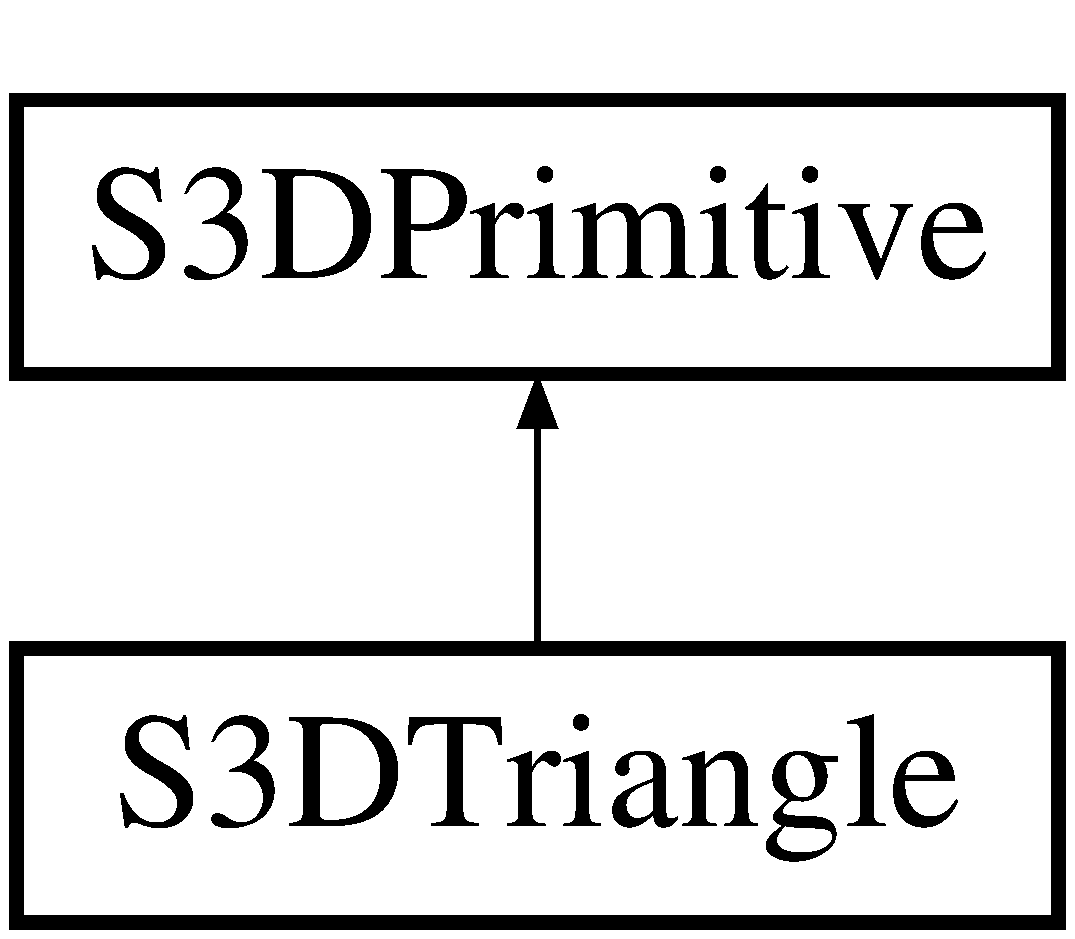
\includegraphics[height=2cm]{class_s3_d_triangle}
\end{center}
\end{figure}
\subsection*{Public Member Functions}
\begin{DoxyCompactItemize}
\item 
\hyperlink{class_s3_d_triangle_a2ac27d0814934c422e3fbf593c77014e}{S3DTriangle} (\hyperlink{class_s3_d_point}{S3DPoint} points\mbox{[}3\mbox{]})
\begin{DoxyCompactList}\small\item\em Constructor for the triangle. \item\end{DoxyCompactList}\item 
\hyperlink{class_s3_d_triangle_a6709f19586226831dc2a50466e3e669e}{S3DTriangle} (\hyperlink{class_s3_d_point}{S3DPoint} a, \hyperlink{class_s3_d_point}{S3DPoint} b, \hyperlink{class_s3_d_point}{S3DPoint} c)
\begin{DoxyCompactList}\small\item\em Constructor for the triangle. \item\end{DoxyCompactList}\item 
void \hyperlink{class_s3_d_triangle_a7f168122e4ed627fcb6489852a56982b}{move} (double dx, double dy, double dz)
\begin{DoxyCompactList}\small\item\em Moves the triangle (translates it) relative to its coordinates. \item\end{DoxyCompactList}\item 
void \hyperlink{class_s3_d_triangle_a3e739f6c9c176e58cb734db7328cf039}{rotate} (double rx, double ry, double rz, \hyperlink{class_s3_d_point}{S3DPoint} $\ast$anchor=NULL)
\begin{DoxyCompactList}\small\item\em Rotates the triangle around its center or another anchor point. \item\end{DoxyCompactList}\item 
void \hyperlink{class_s3_d_triangle_a0808a047e513fb2322e3fc6465c7c011}{scale} (double fx, double fy, double fz)
\begin{DoxyCompactList}\small\item\em Scales the triangle. \item\end{DoxyCompactList}\item 
void \hyperlink{class_s3_d_triangle_acf6924908c89d6bbc5af23769243beaf}{draw} (S3DDevice $\ast$disp, S3DSurface window, S3DContext gc, \hyperlink{class_s3_d_z_buffer}{S3DZBuffer} $\ast$zbuffer)
\begin{DoxyCompactList}\small\item\em Draws the triangle. \item\end{DoxyCompactList}\item 
void \hyperlink{class_s3_d_triangle_a2c60503c3bae194ec8247a0e2467c915}{setColor} (unsigned long c)
\begin{DoxyCompactList}\small\item\em Sets the color the triangle is drawn in. \item\end{DoxyCompactList}\item 
unsigned long \hyperlink{class_s3_d_triangle_ade8ba96094206ee3dff5c3bc743e0a1c}{getColor} ()
\begin{DoxyCompactList}\small\item\em Returns the color the triangle is drawn in. \item\end{DoxyCompactList}\item 
\hyperlink{class_s3_d_point}{S3DPoint} $\ast$ \hyperlink{class_s3_d_triangle_a1032adb6846335a47c8e8c0355b69dbd}{getPoints} ()
\begin{DoxyCompactList}\small\item\em Returns an array of the points, the triangle is built upon. \item\end{DoxyCompactList}\item 
double \hyperlink{class_s3_d_triangle_a35428b5799c8d51a6c57d1fdb5b575a1}{getZ} ()
\begin{DoxyCompactList}\small\item\em Returns the z-\/coordinate for the center of the triangle. \item\end{DoxyCompactList}\end{DoxyCompactItemize}


\subsection{Detailed Description}
This is the main primitive actually used. This is the mostly used primitive, because all complex primitives base upon triangles. It is platform-\/independent, because all drawing is done using \hyperlink{class_s3_d_line}{S3DLine}. 

\subsection{Constructor \& Destructor Documentation}
\hypertarget{class_s3_d_triangle_a2ac27d0814934c422e3fbf593c77014e}{
\index{S3DTriangle@{S3DTriangle}!S3DTriangle@{S3DTriangle}}
\index{S3DTriangle@{S3DTriangle}!S3DTriangle@{S3DTriangle}}
\subsubsection[{S3DTriangle}]{\setlength{\rightskip}{0pt plus 5cm}S3DTriangle::S3DTriangle ({\bf S3DPoint} {\em points}\mbox{[}3\mbox{]})}}
\label{class_s3_d_triangle_a2ac27d0814934c422e3fbf593c77014e}


Constructor for the triangle. 


\begin{DoxyParams}{Parameters}
\item[\mbox{$\leftarrow$} {\em points}]Array of three S3DPoints, marking the points, the triangle is made of.\end{DoxyParams}
Constructs a new instance of S3Triangle based upon the points supplied. \hypertarget{class_s3_d_triangle_a6709f19586226831dc2a50466e3e669e}{
\index{S3DTriangle@{S3DTriangle}!S3DTriangle@{S3DTriangle}}
\index{S3DTriangle@{S3DTriangle}!S3DTriangle@{S3DTriangle}}
\subsubsection[{S3DTriangle}]{\setlength{\rightskip}{0pt plus 5cm}S3DTriangle::S3DTriangle ({\bf S3DPoint} {\em a}, \/  {\bf S3DPoint} {\em b}, \/  {\bf S3DPoint} {\em c})}}
\label{class_s3_d_triangle_a6709f19586226831dc2a50466e3e669e}


Constructor for the triangle. 


\begin{DoxyParams}{Parameters}
\item[\mbox{$\leftarrow$} {\em a}]First point, the triangle will be build upon. \item[\mbox{$\leftarrow$} {\em b}]Second point, the triangle will be build upon. \item[\mbox{$\leftarrow$} {\em c}]Third point, the triangle will be build upon.\end{DoxyParams}
Constructs a new instance of S3Triangle based upon the points supplied. 

\subsection{Member Function Documentation}
\hypertarget{class_s3_d_triangle_acf6924908c89d6bbc5af23769243beaf}{
\index{S3DTriangle@{S3DTriangle}!draw@{draw}}
\index{draw@{draw}!S3DTriangle@{S3DTriangle}}
\subsubsection[{draw}]{\setlength{\rightskip}{0pt plus 5cm}void S3DTriangle::draw (S3DDevice $\ast$ {\em disp}, \/  S3DSurface {\em window}, \/  S3DContext {\em gc}, \/  {\bf S3DZBuffer} $\ast$ {\em zbuffer})\hspace{0.3cm}{\ttfamily  \mbox{[}virtual\mbox{]}}}}
\label{class_s3_d_triangle_acf6924908c89d6bbc5af23769243beaf}


Draws the triangle. 


\begin{DoxyParams}{Parameters}
\item[\mbox{$\leftarrow$} {\em disp}]The display device, the line will be drawn to \item[\mbox{$\leftarrow$} {\em window}]The surface, the line will be drawn to \item[\mbox{$\leftarrow$} {\em gc}]The context, the line will be drawn to \item[{\em zbuffer}]Pointer to the S3DZBuffer-\/Instance of the Simple3D-\/Instance.\end{DoxyParams}
Draws the triangle by drawing the triangles it consists of. This method does NOT contain platform-\/specific calls anymore, because it uses the underlying triangles to draw the triangle. The meaning and neccessity of disp, window and gc may vary between different platforms 

Implements \hyperlink{class_s3_d_primitive_a857f042bc63ae6233b63b60089e92b81}{S3DPrimitive}.

\hypertarget{class_s3_d_triangle_ade8ba96094206ee3dff5c3bc743e0a1c}{
\index{S3DTriangle@{S3DTriangle}!getColor@{getColor}}
\index{getColor@{getColor}!S3DTriangle@{S3DTriangle}}
\subsubsection[{getColor}]{\setlength{\rightskip}{0pt plus 5cm}unsigned long S3DTriangle::getColor ()}}
\label{class_s3_d_triangle_ade8ba96094206ee3dff5c3bc743e0a1c}


Returns the color the triangle is drawn in. 

\begin{DoxyReturn}{Returns}
Color (unsigned long as produced by the RGB-\/macro) of the triangle. 
\end{DoxyReturn}


Reimplemented from \hyperlink{class_s3_d_primitive_a4102845e7754e44c51a87c0fcb391c73}{S3DPrimitive}.

\hypertarget{class_s3_d_triangle_a1032adb6846335a47c8e8c0355b69dbd}{
\index{S3DTriangle@{S3DTriangle}!getPoints@{getPoints}}
\index{getPoints@{getPoints}!S3DTriangle@{S3DTriangle}}
\subsubsection[{getPoints}]{\setlength{\rightskip}{0pt plus 5cm}{\bf S3DPoint} $\ast$ S3DTriangle::getPoints ()}}
\label{class_s3_d_triangle_a1032adb6846335a47c8e8c0355b69dbd}


Returns an array of the points, the triangle is built upon. 

\begin{DoxyReturn}{Returns}
Array of three S3DPoints. 
\end{DoxyReturn}
\hypertarget{class_s3_d_triangle_a35428b5799c8d51a6c57d1fdb5b575a1}{
\index{S3DTriangle@{S3DTriangle}!getZ@{getZ}}
\index{getZ@{getZ}!S3DTriangle@{S3DTriangle}}
\subsubsection[{getZ}]{\setlength{\rightskip}{0pt plus 5cm}double S3DTriangle::getZ ()\hspace{0.3cm}{\ttfamily  \mbox{[}virtual\mbox{]}}}}
\label{class_s3_d_triangle_a35428b5799c8d51a6c57d1fdb5b575a1}


Returns the z-\/coordinate for the center of the triangle. 

This function is used for Z-\/Buffering and currently also for the painter's algorithm to determine the order in which the entities get drawn. 

Implements \hyperlink{class_s3_d_primitive_ab5b06d3a8e83216cc42554bb78afd2d9}{S3DPrimitive}.

\hypertarget{class_s3_d_triangle_a7f168122e4ed627fcb6489852a56982b}{
\index{S3DTriangle@{S3DTriangle}!move@{move}}
\index{move@{move}!S3DTriangle@{S3DTriangle}}
\subsubsection[{move}]{\setlength{\rightskip}{0pt plus 5cm}void S3DTriangle::move (double {\em dx}, \/  double {\em dy}, \/  double {\em dz})\hspace{0.3cm}{\ttfamily  \mbox{[}virtual\mbox{]}}}}
\label{class_s3_d_triangle_a7f168122e4ed627fcb6489852a56982b}


Moves the triangle (translates it) relative to its coordinates. 


\begin{DoxyParams}{Parameters}
\item[\mbox{$\leftarrow$} {\em dx}]The distance the triangle is moved in x-\/direction \item[\mbox{$\leftarrow$} {\em dy}]The distance the triangle is moved in y-\/direction \item[\mbox{$\leftarrow$} {\em dz}]The distance the triangle is moved in z-\/direction \end{DoxyParams}


Implements \hyperlink{class_s3_d_primitive_a73a178ec2e1aa8e95f01baf0552724a9}{S3DPrimitive}.

\hypertarget{class_s3_d_triangle_a3e739f6c9c176e58cb734db7328cf039}{
\index{S3DTriangle@{S3DTriangle}!rotate@{rotate}}
\index{rotate@{rotate}!S3DTriangle@{S3DTriangle}}
\subsubsection[{rotate}]{\setlength{\rightskip}{0pt plus 5cm}void S3DTriangle::rotate (double {\em rx}, \/  double {\em ry}, \/  double {\em rz}, \/  {\bf S3DPoint} $\ast$ {\em anchor} = {\ttfamily NULL})\hspace{0.3cm}{\ttfamily  \mbox{[}virtual\mbox{]}}}}
\label{class_s3_d_triangle_a3e739f6c9c176e58cb734db7328cf039}


Rotates the triangle around its center or another anchor point. 


\begin{DoxyParams}{Parameters}
\item[\mbox{$\leftarrow$} {\em rx}]The angle the triangle should be rotated around the x-\/axis \item[\mbox{$\leftarrow$} {\em ry}]The angle the triangle should be rotated around the y-\/axis \item[\mbox{$\leftarrow$} {\em rz}]The angle the triangle should be rotated around the z-\/axis \item[\mbox{$\leftarrow$} {\em anchor}]Optional. The point the triangle should be rotated around, instead of its own center.\end{DoxyParams}
This function allows to rotate the triangle around all three axis in any angle. If no anchor-\/point is passed, the triangle will be rotated around its own center, else it will rotate around the given point. 

Implements \hyperlink{class_s3_d_primitive_a23eb36b6bd48643e8f7be4b950592d9e}{S3DPrimitive}.

\hypertarget{class_s3_d_triangle_a0808a047e513fb2322e3fc6465c7c011}{
\index{S3DTriangle@{S3DTriangle}!scale@{scale}}
\index{scale@{scale}!S3DTriangle@{S3DTriangle}}
\subsubsection[{scale}]{\setlength{\rightskip}{0pt plus 5cm}void S3DTriangle::scale (double {\em fx}, \/  double {\em fy}, \/  double {\em fz})}}
\label{class_s3_d_triangle_a0808a047e513fb2322e3fc6465c7c011}


Scales the triangle. 


\begin{DoxyParams}{Parameters}
\item[\mbox{$\leftarrow$} {\em fx}]Scaling factor along the x-\/axis \item[\mbox{$\leftarrow$} {\em fy}]Scaling factor along the y-\/axis \item[\mbox{$\leftarrow$} {\em fz}]Scaling factor along the z-\/axis\end{DoxyParams}
This method scales the triangle according to the given factors internall, its also translated, to preserve its center's coordinates. \begin{Desc}
\item[\hyperlink{todo__todo000002}{Todo}]Currently this works for stand-\/alone triangles, but not for triangles belonging to \hyperlink{class_s3_d_mesh}{S3DMesh}. \end{Desc}
\hypertarget{class_s3_d_triangle_a2c60503c3bae194ec8247a0e2467c915}{
\index{S3DTriangle@{S3DTriangle}!setColor@{setColor}}
\index{setColor@{setColor}!S3DTriangle@{S3DTriangle}}
\subsubsection[{setColor}]{\setlength{\rightskip}{0pt plus 5cm}void S3DTriangle::setColor (unsigned long {\em c})}}
\label{class_s3_d_triangle_a2c60503c3bae194ec8247a0e2467c915}


Sets the color the triangle is drawn in. 


\begin{DoxyParams}{Parameters}
\item[\mbox{$\leftarrow$} {\em c}]Color (unsigned long as produced by the RGB-\/macro) that will be used to draw the triangle. \end{DoxyParams}


Reimplemented from \hyperlink{class_s3_d_primitive_a1c8f036193987522bdfb6a49b9b74000}{S3DPrimitive}.



The documentation for this class was generated from the following files:\begin{DoxyCompactItemize}
\item 
Simple3D/\hyperlink{_s3_d_triangle_8h}{S3DTriangle.h}\item 
Simple3D/\hyperlink{_s3_d_triangle_8cpp}{S3DTriangle.cpp}\end{DoxyCompactItemize}

\hypertarget{class_s3_d_z_buffer}{
\section{S3DZBuffer Class Reference}
\label{class_s3_d_z_buffer}\index{S3DZBuffer@{S3DZBuffer}}
}


This class is responsible for z-\/buffering.  




{\ttfamily \#include $<$S3DZBuffer.h$>$}

\subsection*{Public Member Functions}
\begin{DoxyCompactItemize}
\item 
\hyperlink{class_s3_d_z_buffer_a8983fb4278e5baaa4bdf076f8e28d940}{S3DZBuffer} (int w, int h)
\begin{DoxyCompactList}\small\item\em Default constructor. \item\end{DoxyCompactList}\item 
int \hyperlink{class_s3_d_z_buffer_aba5f79850772a0500a629443e413e402}{getPoint} (int x, int y)
\begin{DoxyCompactList}\small\item\em Gets the z-\/buffer value for the given coordinates. \item\end{DoxyCompactList}\item 
void \hyperlink{class_s3_d_z_buffer_aa712e633bf2ccf4c43bb27178a1692c1}{setPoint} (int x, int y, int z)
\begin{DoxyCompactList}\small\item\em Sets the z-\/buffer value for the given coordinates. \item\end{DoxyCompactList}\item 
void \hyperlink{class_s3_d_z_buffer_ab2b22d8f910724846765813cc6e8457e}{clear} ()
\begin{DoxyCompactList}\small\item\em Clears the z-\/buffer. \item\end{DoxyCompactList}\end{DoxyCompactItemize}


\subsection{Detailed Description}
This class is responsible for z-\/buffering. This class is the foundation of the z-\/buffering. Its used to determine, if a pixel should be drawn or not and is used in \hyperlink{class_s3_d_line}{S3DLine} and \hyperlink{class_s3_d_point}{S3DPoint} to check and update the z-\/buffer, before/after the actual drawing. \hyperlink{class_simple3_d}{Simple3D} manages to keep the z-\/buffer clean and passes the reference to the entities. 

\subsection{Constructor \& Destructor Documentation}
\hypertarget{class_s3_d_z_buffer_a8983fb4278e5baaa4bdf076f8e28d940}{
\index{S3DZBuffer@{S3DZBuffer}!S3DZBuffer@{S3DZBuffer}}
\index{S3DZBuffer@{S3DZBuffer}!S3DZBuffer@{S3DZBuffer}}
\subsubsection[{S3DZBuffer}]{\setlength{\rightskip}{0pt plus 5cm}S3DZBuffer::S3DZBuffer (int {\em w}, \/  int {\em h})}}
\label{class_s3_d_z_buffer_a8983fb4278e5baaa4bdf076f8e28d940}


Default constructor. 


\begin{DoxyParams}{Parameters}
\item[\mbox{$\leftarrow$} {\em w}]Width of the buffer (i.e. width of the screen) \item[\mbox{$\leftarrow$} {\em h}]Height of the buffer (i.e. height of the screen)\end{DoxyParams}
The constructor is called from within \hyperlink{class_simple3_d}{Simple3D} on initialization. You should not call it yourself. 

\subsection{Member Function Documentation}
\hypertarget{class_s3_d_z_buffer_ab2b22d8f910724846765813cc6e8457e}{
\index{S3DZBuffer@{S3DZBuffer}!clear@{clear}}
\index{clear@{clear}!S3DZBuffer@{S3DZBuffer}}
\subsubsection[{clear}]{\setlength{\rightskip}{0pt plus 5cm}void S3DZBuffer::clear ()}}
\label{class_s3_d_z_buffer_ab2b22d8f910724846765813cc6e8457e}


Clears the z-\/buffer. 

\hypertarget{class_s3_d_z_buffer_aba5f79850772a0500a629443e413e402}{
\index{S3DZBuffer@{S3DZBuffer}!getPoint@{getPoint}}
\index{getPoint@{getPoint}!S3DZBuffer@{S3DZBuffer}}
\subsubsection[{getPoint}]{\setlength{\rightskip}{0pt plus 5cm}int S3DZBuffer::getPoint (int {\em x}, \/  int {\em y})}}
\label{class_s3_d_z_buffer_aba5f79850772a0500a629443e413e402}


Gets the z-\/buffer value for the given coordinates. 


\begin{DoxyParams}{Parameters}
\item[\mbox{$\leftarrow$} {\em x}]The x-\/coordinate of the point on screen \item[\mbox{$\leftarrow$} {\em y}]The y-\/coordinate of the point on screen \end{DoxyParams}
\begin{DoxyReturn}{Returns}
The z-\/Buffer value (i.e. the z-\/coordinate of the drawn point) for the coordinates (x,y) 
\end{DoxyReturn}
\hypertarget{class_s3_d_z_buffer_aa712e633bf2ccf4c43bb27178a1692c1}{
\index{S3DZBuffer@{S3DZBuffer}!setPoint@{setPoint}}
\index{setPoint@{setPoint}!S3DZBuffer@{S3DZBuffer}}
\subsubsection[{setPoint}]{\setlength{\rightskip}{0pt plus 5cm}void S3DZBuffer::setPoint (int {\em x}, \/  int {\em y}, \/  int {\em z})}}
\label{class_s3_d_z_buffer_aa712e633bf2ccf4c43bb27178a1692c1}


Sets the z-\/buffer value for the given coordinates. 


\begin{DoxyParams}{Parameters}
\item[\mbox{$\leftarrow$} {\em x}]The x-\/coordinate of the point on screen \item[\mbox{$\leftarrow$} {\em y}]The y-\/coordinate of the point on screen \item[\mbox{$\leftarrow$} {\em z}]The z-\/value of the point on screen \end{DoxyParams}


The documentation for this class was generated from the following files:\begin{DoxyCompactItemize}
\item 
\hyperlink{_s3_d_z_buffer_8h}{S3DZBuffer.h}\item 
\hyperlink{_s3_d_z_buffer_8cpp}{S3DZBuffer.cpp}\end{DoxyCompactItemize}

\hypertarget{class_simple3_d}{
\section{Simple3D Class Reference}
\label{class_simple3_d}\index{Simple3D@{Simple3D}}
}


This class is the main class of the engine.  




{\ttfamily \#include $<$Simple3D.h$>$}

\subsection*{Public Member Functions}
\begin{DoxyCompactItemize}
\item 
\hyperlink{class_simple3_d_a7644ace43261dd71e7f3cb9c9659025d}{Simple3D} (int width, int height, std::string title, int argc=0, char $\ast$$\ast$argv=0)
\begin{DoxyCompactList}\small\item\em The default constructor. You need to call this to initialize the engine. \item\end{DoxyCompactList}\item 
\hypertarget{class_simple3_d_a859666c712fd07748e9fca5938bbfa55}{
\hyperlink{class_simple3_d_a859666c712fd07748e9fca5938bbfa55}{$\sim$Simple3D} ()}
\label{class_simple3_d_a859666c712fd07748e9fca5938bbfa55}

\begin{DoxyCompactList}\small\item\em Destructor. Call this to clean up after you're ready with S3D. \item\end{DoxyCompactList}\item 
void \hyperlink{class_simple3_d_abe4d7beed767d1d24154738fad7ac1a7}{appendEntity} (\hyperlink{class_s3_d_primitive}{S3DPrimitive} $\ast$p)
\begin{DoxyCompactList}\small\item\em Propagate entity to the engine. \item\end{DoxyCompactList}\item 
void \hyperlink{class_simple3_d_ab98d8b6cfb6abf91b43a035ab36f75f8}{render} ()
\begin{DoxyCompactList}\small\item\em Renders the entities known to the instance of \hyperlink{class_simple3_d}{Simple3D}. \item\end{DoxyCompactList}\item 
void \hyperlink{class_simple3_d_a2e1f61afda5ab9cb2a1abd05a856c5d7}{setBackColor} (\hyperlink{struct_s3_d_color}{S3DColor} c)
\begin{DoxyCompactList}\small\item\em Set the background color. \item\end{DoxyCompactList}\item 
void \hyperlink{class_simple3_d_a9dd0eb5a220c4490656dc3dd5cc79857}{setForeColor} (\hyperlink{struct_s3_d_color}{S3DColor} c)
\begin{DoxyCompactList}\small\item\em Set the background color. \item\end{DoxyCompactList}\item 
S3DEvent \hyperlink{class_simple3_d_a8f6621e3e0b4bfae3011514e7fc73003}{getEvent} ()
\begin{DoxyCompactList}\small\item\em Obtain an event from the engine's window. \item\end{DoxyCompactList}\item 
void \hyperlink{class_simple3_d_aa0da52599eafb396ec36e3d0cf6da504}{reOrderEntities} ()
\begin{DoxyCompactList}\small\item\em Reorders entities for correct rendering. \item\end{DoxyCompactList}\end{DoxyCompactItemize}


\subsection{Detailed Description}
This class is the main class of the engine. You need to create an instance of this class to use the engine. It manages the platform-\/specific things on initialization, handles events and renders primitives to screen. 

\subsection{Constructor \& Destructor Documentation}
\hypertarget{class_simple3_d_a7644ace43261dd71e7f3cb9c9659025d}{
\index{Simple3D@{Simple3D}!Simple3D@{Simple3D}}
\index{Simple3D@{Simple3D}!Simple3D@{Simple3D}}
\subsubsection[{Simple3D}]{\setlength{\rightskip}{0pt plus 5cm}Simple3D::Simple3D (int {\em width}, \/  int {\em height}, \/  std::string {\em title}, \/  int {\em argc} = {\ttfamily 0}, \/  char $\ast$$\ast$ {\em argv} = {\ttfamily 0})}}
\label{class_simple3_d_a7644ace43261dd71e7f3cb9c9659025d}


The default constructor. You need to call this to initialize the engine. 


\begin{DoxyParams}{Parameters}
\item[\mbox{$\leftarrow$} {\em width}]The width of the desired screen. \item[\mbox{$\leftarrow$} {\em height}]The height of the desired screen. \item[\mbox{$\leftarrow$} {\em title}]You can supply a title for a window here. \item[\mbox{$\leftarrow$} {\em argc}]The number of arguments passed to your application (optional) \item[\mbox{$\leftarrow$} {\em argv}]The arguments passed to your application (optional) \end{DoxyParams}


\subsection{Member Function Documentation}
\hypertarget{class_simple3_d_abe4d7beed767d1d24154738fad7ac1a7}{
\index{Simple3D@{Simple3D}!appendEntity@{appendEntity}}
\index{appendEntity@{appendEntity}!Simple3D@{Simple3D}}
\subsubsection[{appendEntity}]{\setlength{\rightskip}{0pt plus 5cm}void Simple3D::appendEntity ({\bf S3DPrimitive} $\ast$ {\em p})}}
\label{class_simple3_d_abe4d7beed767d1d24154738fad7ac1a7}


Propagate entity to the engine. 


\begin{DoxyParams}{Parameters}
\item[\mbox{$\leftarrow$} {\em p}]Pointer to the primitive you want to enqueue for rendering.\end{DoxyParams}
You need to call this function in order to get an entity on screen. Only entities enqueued through this function are rendered. \hypertarget{class_simple3_d_a8f6621e3e0b4bfae3011514e7fc73003}{
\index{Simple3D@{Simple3D}!getEvent@{getEvent}}
\index{getEvent@{getEvent}!Simple3D@{Simple3D}}
\subsubsection[{getEvent}]{\setlength{\rightskip}{0pt plus 5cm}S3DEvent Simple3D::getEvent ()}}
\label{class_simple3_d_a8f6621e3e0b4bfae3011514e7fc73003}


Obtain an event from the engine's window. 

\begin{DoxyReturn}{Returns}
Returns an S3DEvent-\/structure. When there was no event, S3DEventNone is returned. 
\end{DoxyReturn}
\hypertarget{class_simple3_d_ab98d8b6cfb6abf91b43a035ab36f75f8}{
\index{Simple3D@{Simple3D}!render@{render}}
\index{render@{render}!Simple3D@{Simple3D}}
\subsubsection[{render}]{\setlength{\rightskip}{0pt plus 5cm}void Simple3D::render ()}}
\label{class_simple3_d_ab98d8b6cfb6abf91b43a035ab36f75f8}


Renders the entities known to the instance of \hyperlink{class_simple3_d}{Simple3D}. 

You need to call this, when you want to render the entities, you have propagated to the engine-\/instance. \hypertarget{class_simple3_d_aa0da52599eafb396ec36e3d0cf6da504}{
\index{Simple3D@{Simple3D}!reOrderEntities@{reOrderEntities}}
\index{reOrderEntities@{reOrderEntities}!Simple3D@{Simple3D}}
\subsubsection[{reOrderEntities}]{\setlength{\rightskip}{0pt plus 5cm}void Simple3D::reOrderEntities ()}}
\label{class_simple3_d_aa0da52599eafb396ec36e3d0cf6da504}


Reorders entities for correct rendering. 

This gets called from inside the engine. You don't need to fiddle with this. \hypertarget{class_simple3_d_a2e1f61afda5ab9cb2a1abd05a856c5d7}{
\index{Simple3D@{Simple3D}!setBackColor@{setBackColor}}
\index{setBackColor@{setBackColor}!Simple3D@{Simple3D}}
\subsubsection[{setBackColor}]{\setlength{\rightskip}{0pt plus 5cm}void Simple3D::setBackColor ({\bf S3DColor} {\em c})}}
\label{class_simple3_d_a2e1f61afda5ab9cb2a1abd05a856c5d7}


Set the background color. 


\begin{DoxyParams}{Parameters}
\item[\mbox{$\leftarrow$} {\em c}]Color (unsigned int as produced by the RGB-\/macro) to use as background.\end{DoxyParams}
Call this to set the color used by the engine as background. Default color is black. \hypertarget{class_simple3_d_a9dd0eb5a220c4490656dc3dd5cc79857}{
\index{Simple3D@{Simple3D}!setForeColor@{setForeColor}}
\index{setForeColor@{setForeColor}!Simple3D@{Simple3D}}
\subsubsection[{setForeColor}]{\setlength{\rightskip}{0pt plus 5cm}void Simple3D::setForeColor ({\bf S3DColor} {\em c})}}
\label{class_simple3_d_a9dd0eb5a220c4490656dc3dd5cc79857}


Set the background color. 


\begin{DoxyParams}{Parameters}
\item[\mbox{$\leftarrow$} {\em c}]Color (unsigned int as produced by the RGB-\/macro) to use as background.\end{DoxyParams}
Call this to set the color used by the engine for rendering, when no other color is specified. Default color is white. Note: The axis are (if displayed) drawn in this color. 

The documentation for this class was generated from the following files:\begin{DoxyCompactItemize}
\item 
Simple3D/\hyperlink{_simple3_d_8h}{Simple3D.h}\item 
Simple3D/\hyperlink{_simple3_d_8cpp}{Simple3D.cpp}\end{DoxyCompactItemize}

\chapter{File Documentation}
\hypertarget{global_8h}{
\section{global.h File Reference}
\label{global_8h}\index{global.h@{global.h}}
}


Contains basic includes (including platform-\/dependent) and definitions for the whole library.  


{\ttfamily \#include $<$cstdlib$>$}\par
{\ttfamily \#include $<$X11/Xlib.h$>$}\par
{\ttfamily \#include $<$X11/Xutil.h$>$}\par
{\ttfamily \#include $<$X11/Xos.h$>$}\par
{\ttfamily \#include \char`\"{}types.h\char`\"{}}\par
\subsection*{Defines}
\begin{DoxyCompactItemize}
\item 
\#define \hyperlink{global_8h_a598a3330b3c21701223ee0ca14316eca}{PI}~3.14159
\item 
\#define \hyperlink{global_8h_a4a118ad3ee36468a3fa616977a64864e}{RGB}(r, g, b)~((r $<$$<$ 16) $|$ (g $<$$<$ 8) $|$ b)
\item 
\#define \hyperlink{global_8h_a7566fab7adbea8a8499b8e231550d26c}{PLANAR\_\-DISTANCE}~300
\end{DoxyCompactItemize}


\subsection{Detailed Description}
Contains basic includes (including platform-\/dependent) and definitions for the whole library. 

\subsection{Define Documentation}
\hypertarget{global_8h_a598a3330b3c21701223ee0ca14316eca}{
\index{global.h@{global.h}!PI@{PI}}
\index{PI@{PI}!global.h@{global.h}}
\subsubsection[{PI}]{\setlength{\rightskip}{0pt plus 5cm}\#define PI~3.14159}}
\label{global_8h_a598a3330b3c21701223ee0ca14316eca}
\hypertarget{global_8h_a7566fab7adbea8a8499b8e231550d26c}{
\index{global.h@{global.h}!PLANAR\_\-DISTANCE@{PLANAR\_\-DISTANCE}}
\index{PLANAR\_\-DISTANCE@{PLANAR\_\-DISTANCE}!global.h@{global.h}}
\subsubsection[{PLANAR\_\-DISTANCE}]{\setlength{\rightskip}{0pt plus 5cm}\#define PLANAR\_\-DISTANCE~300}}
\label{global_8h_a7566fab7adbea8a8499b8e231550d26c}
\hypertarget{global_8h_a4a118ad3ee36468a3fa616977a64864e}{
\index{global.h@{global.h}!RGB@{RGB}}
\index{RGB@{RGB}!global.h@{global.h}}
\subsubsection[{RGB}]{\setlength{\rightskip}{0pt plus 5cm}\#define RGB(r, \/  g, \/  b)~((r $<$$<$ 16) $|$ (g $<$$<$ 8) $|$ b)}}
\label{global_8h_a4a118ad3ee36468a3fa616977a64864e}

\hypertarget{_s3_d_line_8cpp}{
\section{S3DLine.cpp File Reference}
\label{_s3_d_line_8cpp}\index{S3DLine.cpp@{S3DLine.cpp}}
}


Contains the implementation of the S3DLine-\/Primitive.  


{\ttfamily \#include \char`\"{}S3DLine.h\char`\"{}}\par


\subsection{Detailed Description}
Contains the implementation of the S3DLine-\/Primitive. 
\hypertarget{_s3_d_line_8h}{
\section{S3DLine.h File Reference}
\label{_s3_d_line_8h}\index{S3DLine.h@{S3DLine.h}}
}


Contains the class-\/definition (and getter and setter) for \hyperlink{class_s3_d_line}{S3DLine}.  


{\ttfamily \#include $<$iostream$>$}\par
{\ttfamily \#include \char`\"{}S3DPrimitive.h\char`\"{}}\par
{\ttfamily \#include \char`\"{}S3DPoint.h\char`\"{}}\par
\subsection*{Classes}
\begin{DoxyCompactItemize}
\item 
class \hyperlink{class_s3_d_line}{S3DLine}
\begin{DoxyCompactList}\small\item\em Class for the line-\/primitive in S3D. \item\end{DoxyCompactList}\end{DoxyCompactItemize}


\subsection{Detailed Description}
Contains the class-\/definition (and getter and setter) for \hyperlink{class_s3_d_line}{S3DLine}. 
\hypertarget{_s3_d_mesh_8cpp}{
\section{S3DMesh.cpp File Reference}
\label{_s3_d_mesh_8cpp}\index{S3DMesh.cpp@{S3DMesh.cpp}}
}


Contains the code for loading an entity from a file and use it.  


{\ttfamily \#include \char`\"{}S3DMesh.h\char`\"{}}\par


\subsection{Detailed Description}
Contains the code for loading an entity from a file and use it. 
\hypertarget{_s3_d_mesh_8h}{
\section{S3DMesh.h File Reference}
\label{_s3_d_mesh_8h}\index{S3DMesh.h@{S3DMesh.h}}
}
{\ttfamily \#include $<$fstream$>$}\par
{\ttfamily \#include $<$vector$>$}\par
{\ttfamily \#include $<$iostream$>$}\par
{\ttfamily \#include \char`\"{}S3DTriangle.h\char`\"{}}\par
\subsection*{Classes}
\begin{DoxyCompactItemize}
\item 
class \hyperlink{class_s3_d_mesh}{S3DMesh}
\begin{DoxyCompactList}\small\item\em This class is used to load a collection of triangles to use it as an entity. \item\end{DoxyCompactList}\end{DoxyCompactItemize}


\subsection{Detailed Description}
Contains declarations for \hyperlink{class_s3_d_mesh}{S3DMesh} 
\hypertarget{_s3_d_point_8cpp}{
\section{Simple3D/S3DPoint.cpp File Reference}
\label{_s3_d_point_8cpp}\index{Simple3D/S3DPoint.cpp@{Simple3D/S3DPoint.cpp}}
}
{\ttfamily \#include \char`\"{}S3DPoint.h\char`\"{}}\par


\subsection{Detailed Description}
Contains the implementation of \hyperlink{class_s3_d_point}{S3DPoint} 
\hypertarget{_s3_d_point_8h}{
\section{S3DPoint.h File Reference}
\label{_s3_d_point_8h}\index{S3DPoint.h@{S3DPoint.h}}
}


Contains definitions of \hyperlink{class_s3_d_point}{S3DPoint}.  


{\ttfamily \#include \char`\"{}global.h\char`\"{}}\par
\subsection*{Classes}
\begin{DoxyCompactItemize}
\item 
class \hyperlink{class_s3_d_point}{S3DPoint}
\begin{DoxyCompactList}\small\item\em This class is used for representing 3d-\/coordinates. \item\end{DoxyCompactList}\end{DoxyCompactItemize}


\subsection{Detailed Description}
Contains definitions of \hyperlink{class_s3_d_point}{S3DPoint}. 
\hypertarget{_s3_d_primitive_8cpp}{
\section{S3DPrimitive.cpp File Reference}
\label{_s3_d_primitive_8cpp}\index{S3DPrimitive.cpp@{S3DPrimitive.cpp}}
}


Contains the code for \hyperlink{class_s3_d_primitive}{S3DPrimitive}.  


{\ttfamily \#include \char`\"{}S3DPrimitive.h\char`\"{}}\par


\subsection{Detailed Description}
Contains the code for \hyperlink{class_s3_d_primitive}{S3DPrimitive}. 
\hypertarget{_s3_d_primitive_8h}{
\section{Simple3D/S3DPrimitive.h File Reference}
\label{_s3_d_primitive_8h}\index{Simple3D/S3DPrimitive.h@{Simple3D/S3DPrimitive.h}}
}
{\ttfamily \#include $<$vector$>$}\par
{\ttfamily \#include \char`\"{}global.h\char`\"{}}\par
{\ttfamily \#include \char`\"{}S3DPoint.h\char`\"{}}\par
{\ttfamily \#include \char`\"{}S3DZBuffer.h\char`\"{}}\par
\subsection*{Classes}
\begin{DoxyCompactItemize}
\item 
class \hyperlink{class_s3_d_primitive}{S3DPrimitive}
\begin{DoxyCompactList}\small\item\em This class is the base of all primitives in S3D. \item\end{DoxyCompactList}\end{DoxyCompactItemize}


\subsection{Detailed Description}
Contains the definition of \hyperlink{class_s3_d_primitive}{S3DPrimitive} 
\hypertarget{_s3_d_triangle_8cpp}{
\section{S3DTriangle.cpp File Reference}
\label{_s3_d_triangle_8cpp}\index{S3DTriangle.cpp@{S3DTriangle.cpp}}
}


Contains the implementation of \hyperlink{class_s3_d_triangle}{S3DTriangle}.  


{\ttfamily \#include \char`\"{}S3DTriangle.h\char`\"{}}\par


\subsection{Detailed Description}
Contains the implementation of \hyperlink{class_s3_d_triangle}{S3DTriangle}. 
\hypertarget{_s3_d_triangle_8h}{
\section{Simple3D/S3DTriangle.h File Reference}
\label{_s3_d_triangle_8h}\index{Simple3D/S3DTriangle.h@{Simple3D/S3DTriangle.h}}
}
{\ttfamily \#include \char`\"{}S3DPoint.h\char`\"{}}\par
{\ttfamily \#include \char`\"{}S3DPrimitive.h\char`\"{}}\par
{\ttfamily \#include \char`\"{}S3DLine.h\char`\"{}}\par
{\ttfamily \#include \char`\"{}S3DZBuffer.h\char`\"{}}\par
\subsection*{Classes}
\begin{DoxyCompactItemize}
\item 
class \hyperlink{class_s3_d_triangle}{S3DTriangle}
\begin{DoxyCompactList}\small\item\em This is the main primitive actually used. \item\end{DoxyCompactList}\end{DoxyCompactItemize}


\subsection{Detailed Description}
Contains the definition for \hyperlink{class_s3_d_triangle}{S3DTriangle}. 
\hypertarget{_s3_d_z_buffer_8h}{
\section{S3DZBuffer.h File Reference}
\label{_s3_d_z_buffer_8h}\index{S3DZBuffer.h@{S3DZBuffer.h}}
}
{\ttfamily \#include \char`\"{}global.h\char`\"{}}\par
\subsection*{Classes}
\begin{DoxyCompactItemize}
\item 
class \hyperlink{class_s3_d_z_buffer}{S3DZBuffer}
\begin{DoxyCompactList}\small\item\em This class is responsible for z-\/buffering. \item\end{DoxyCompactList}\end{DoxyCompactItemize}


\subsection{Detailed Description}
Contains implementation of the \hyperlink{class_s3_d_z_buffer}{S3DZBuffer}

Contains the definition of \hyperlink{class_s3_d_z_buffer}{S3DZBuffer}. 
\hypertarget{_simple3_d_8cpp}{
\section{Simple3D/Simple3D.cpp File Reference}
\label{_simple3_d_8cpp}\index{Simple3D/Simple3D.cpp@{Simple3D/Simple3D.cpp}}
}
{\ttfamily \#include \char`\"{}Simple3D.h\char`\"{}}\par


\subsection{Detailed Description}
Contains the implementation of S3D's core. 
\hypertarget{_simple3_d_8h}{
\section{Simple3D/Simple3D.h File Reference}
\label{_simple3_d_8h}\index{Simple3D/Simple3D.h@{Simple3D/Simple3D.h}}
}
{\ttfamily \#include $<$string$>$}\par
{\ttfamily \#include $<$list$>$}\par
{\ttfamily \#include \char`\"{}global.h\char`\"{}}\par
{\ttfamily \#include \char`\"{}S3DZBuffer.h\char`\"{}}\par
{\ttfamily \#include \char`\"{}S3DMesh.h\char`\"{}}\par
{\ttfamily \#include \char`\"{}S3DLine.h\char`\"{}}\par
\subsection*{Classes}
\begin{DoxyCompactItemize}
\item 
class \hyperlink{class_simple3_d}{Simple3D}
\begin{DoxyCompactList}\small\item\em This class is the main class of the engine. \item\end{DoxyCompactList}\end{DoxyCompactItemize}


\subsection{Detailed Description}
Contains the engine's main class definitions. 
\printindex
\end{document}
